\documentclass[12pt]{article}
\usepackage{lmodern}
\usepackage{hyperref}
\usepackage{setspace}
\usepackage{float}
\hypersetup{
	colorlinks,
	citecolor=black,
	filecolor=black,
	linkcolor=black,
	urlcolor=black	
}
\usepackage{longtable}
\usepackage{amsmath}
\usepackage{listings}
\usepackage{graphicx}
\usepackage{subcaption} 
\usepackage{caption}
\usepackage{geometry}
\usepackage{enumerate}
\usepackage{array, booktabs}  
%\usepackage{multirow}
%\usepackage{tabularx}
\geometry{
	a4paper ,
	total={170mm,257mm},
	left=23mm,
	top=25mm,
	bottom = 25mm,
	right = 23mm
}	
\usepackage{fancyhdr}
\usepackage{gensymb}
\pagestyle{fancy}
\DeclareGraphicsExtensions{.jpg,.png,.pdf}

\usepackage{anyfontsize}

\lhead{}
\chead {ANLP Assignment 1}
\rhead{}
\cfoot{\thepage}

\usepackage[utf8]{inputenc}
\usepackage{color}

\definecolor{deepblue}{rgb}{0,0,0.5}
\definecolor{deepred}{rgb}{0.6,0,0}
\definecolor{deepgreen}{rgb}{0,0.5,0}
% Python style for highlighting


% Default fixed font does not support bold face
\DeclareFixedFont{\ttb}{T1}{txtt}{bx}{n}{12} % for bold
\DeclareFixedFont{\ttm}{T1}{txtt}{m}{n}{12}  % for normal

\newcommand\pythonstyle{\lstset{
		language=Python,
		basicstyle=\ttm,
		otherkeywords={self},             % Add keywords here
		keywordstyle=\ttb\color{deepgreen},
		emph={isEngAlpha,preprocess_line},          % Custom highlighting
		emphstyle=\ttb\color{deepblue},    % Custom highlighting style
		stringstyle=\color{deepred},
		frame=tb,                         % Any extra options here
		showstringspaces=false            % 
}}


% Python environment
\lstnewenvironment{python}[1][]
{
	\pythonstyle
	\lstset{#1}
}
{}


\usepackage{algorithm}
\usepackage[noend]{algpseudocode}

\makeatletter
\def\BState{\State\hskip-\ALG@thistlm}
\makeatother

\usepackage[nottoc,numbib]{tocbibind}


\setlength{\tabcolsep}{18pt}
\renewcommand{\arraystretch}{1.5}

\setcounter{section}{-1} 
\newcolumntype{C}[1]{>{\centering\arraybackslash}p{#1}}

\begin{document}	
	
\begin{titlepage}
	\newcommand{\HRule}{\rule{\linewidth}{0.5mm}} % Defines a new command for the horizontal lines, change thickness here
	\center % Center everything on the page
	\includegraphics[width = 0.3 \linewidth]{"./graphics/avatar-roundel-blackonwhite"}\\[0.5cm]
	\textsc{\\[1cm]\LARGE ACCELERATED NATURAL LANGUAGE \\
             \hfill\break PROCESSING}\\[2cm]

	\HRule \\[0.4cm]
	{ \huge \bfseries Assignment 1}\\[0.1cm]
	\HRule \\[1.5cm]
	\Large
	\vfill
	 s1818699, s1884908\\[0.5cm]
	{\large October 2018}
\end{titlepage}
\setlength\parindent{0pt}		
\newpage
\onehalfspacing
\tableofcontents
\singlespacing
\newpage
	
\section{Introduction}
The main scope of this assignment was to build trigram character models, and use them to produce random output or analyze text perplexity.  This report details the methodology followed to achieve these aims, and includes a discussion of the results obtained throughout the process.
\section{Preprocessing Input File - Question 1}
\label{PreProc}
\subsection{Code}
The code in Listing \ref{pp} demonstrates the methodology used to preprocess input lines.
\begin{python}[caption = {Line Preprocessing},label = {pp}]
def isEngAlpha(character):
#checks if character is specifically english
	if (character >= 'a' and character <= 'z'):
		return True
	elif (character >= 'A' and character <= 'Z'):
		return True
	else:
		return False

def preprocess_line(line):
#Preprocessing of an input line
	character_list = list()
	for character in line:
		if (isEngAlpha(character)): #english checker
			character_list.append(character.lower()) 
		elif (character.isspace() or character == "."): 
			character_list.append(character) #keep ' ','.'
		elif (character.isdigit()):
			# convert digits {0-9} to 0
			character_list.append('0') 
	line = "".join(character_list).rstrip('\n') # remove newline  
	line = '#'+line+'#' #adds sentence start/end markers
	return line
\end{python}
\subsection{Additional Steps in Preprocessing}
Besides removing the illegal characters from each input line as per the specification, a `\#' character has been added to the beginning and ending of each line. This preprocessing step has been adopted in order to also gather trigrams using the beginning/ending (represented as `\#'s) of lines as input characters.  This way, information on sentence starts/ends is not lost, and is quantified through the use of the `\#' markers.  Otherwise, the system would only have been able to begin estimating trigrams from the third character onwards, for every line.  \\
\hfill\break
With this system in place, each line is clearly delimited as a separate sequence.  Characters occurring at the beginning of a sentence (as seen later on in this report) will have a `\#\#' bigram input (indicating a line start), whilst the second character of a sentence will have a `\#\_' bigram input. \\
\hfill\break
Additionally, the newline character `\textbackslash n' at the end of each line has also been removed, to allow for a smooth flow between lines when building n-gram models, without the need for catering for the extra `\textbackslash n'.
\subsection{Sample Input and Output}
A sample input/output pair from the preprocessing function is provided below:\\
\hfill\break
Sample Input: Reanudación del período de sesiones\\
Sample Output: \#reanudacin del perodo de sesiones\#
\section{Determining the Given Model's Estimation Method - Question 2} 
The given language model file contains a number of trigrams followed by the probability of the third character given the first two characters (bigram) in the trigram. To make an assessment of the kind of estimation method used, consider trigrams beginning with `zz'. In English, words containing a `zz' are very rare. Hence the probabilities of such trigrams should all be low and mostly close to zero. On examining the model trigram probabilities beginning with `zz', it has been observed that all such trigrams have a probability of $3.333 * 10^{-2}$.  This immediately indicates that some sort of smoothing has been used to remove all zero probabilities from the model.\\
\hfill\break
One could assume that the model has been smoothed using the Add-Alpha (or Add-One) method. The formula for Add-Alpha smoothing is provided in Equation \ref{AA}.
\begin{equation}\label{AA}
 \dfrac{{count(c_{1},c_{2},c_{3})} + \alpha} {\sum count(c_1,c_2)+ \alpha * |V|} 
\end{equation}\\  
$(c_1,c_2,c_3)$ refer to the first, second and third characters respectively in the trigram, $\alpha$ is a tunable parameter between 0 and 1 and $|V|$ is the size of the vocabulary (i.e. all possible trigrams given the input bigram).\\
\hfill\break
When count $(c_1,c_2,c_3)$ = 0 and count $(c_1,c_2,)$ = 0, Equation \ref{AA} reduces to:

\[\dfrac{1} {|V|} \]

In this case $|V|$ = 30 because the given model character set $ \in \{  \  ,.,0,\#,a,b,c,d,e,f,g,h,i,\\k,l,m,n,o,p,q,r,s,t,u,v,w,x,y,z\}$, hence:

\[\dfrac{1} {|V|}  = \dfrac{1} {30} = 3.33 * 10^{-2}\]

Thus, one could conclude that either Add-One or Add-Alpha smoothing technique has been applied for the model probability estimation. However, when attempting to decipher which value of $\alpha$ has been used, things become more difficult.\\
\hfill\break
Consider another set of rare trigrams beginning with `zy' . The model indicates $p(zy\ | zy) = p(zy. | zy)$ = $3 * 10^{-1}$ whilst all other trigrams beginning with `zy' have a probability of $1.429 * 10^{-2}$. Assuming these other trigrams all have a count of 0, Equation \ref{AA}  would reduce to:
\[\dfrac{ \alpha} {\sum count(zy)+ \alpha * 30} = 1.429 * 10^{-2}\]

This equation has two unknowns:  $\alpha$ and $\sum count(zy)$. The counts of `zy ' and `zy.' are not known. Hence we cannot exactly determine the value of $\alpha$ mathematically.  Plugging in an arbitrary value of $\alpha$ would make sense for these trigrams, but might not make sense for the rest of the trigrams in the model.  One would need to model many simultaneous equations to attempt a guess at the correct value of $\alpha$. \\
\hfill\break
Most other types of estimation are highly improbable in this case.  It certainly cannot be interpolation due to the fact that for all trigrams starting with `zz', the probabilities are uniform.  It is expected that with interpolation, all probabilities for the `zz'-starting trigrams should differ according to the counts of the last character in the trigram (due to its dependence on unigram probabilities).  It is possible that Good-Turing smoothing has been used, but this does not explain the probabilities assigned to the `zz'-starting trigrams since these are all uniform, indicating the same number of counts for each - a problem which simple Good-Turing smoothing cannot deal with.  The uniformity of these low-probability trigrams points to a simpler method of estimation having been used.\\
\hfill\break
Thus, one can conclude with some certainty that either Add-Alpha or Add-One smoothing has been applied within this model for trigram probability estimation. Add-One smoothing is the case where $\alpha$ is set to one, and so Equation \ref{AA} would simply reduce to Equation \ref{A1}, which still fits within our hypothesis.
\begin{equation}\label{A1}
\dfrac{{count(c_{1},c_{2},c_{3})} + \alpha} {\sum count(c_1,c_2)+ \alpha * |V|} = \dfrac{{count(c_{1},c_{2},c_{3})} + 1} {\sum count(c_1,c_2)+ 1 * |V|}  = \dfrac{{count(c_{1},c_{2},c_{3})} + 1} {\sum count(c_1,c_2)+  |V|}
\end{equation}


\section{Trigram Character Language Model - Question 3}
This section contains a description of how trigrams probabilities were collected and estimated, along with an excerpt obtained from the generated language model.
\subsection{Trigram Probability Estimation Method}
The process followed to count and collect raw trigram probabilities is provided below:
\begin{enumerate}
\item Each trigram appearing within the input document is counted and stored within a Python dictionary.  As discussed in Section \ref{PreProc}, an input document is first pre-processed line-by-line before counting occurs.  `\#'s are added at the beginning and end of sentences, in order to signify the start/end of a sequence.  Thus, characters at the beginning of sentences will have a `\#\#' or `\#\_' as their input bigrams.
\item Alongside trigram collection, the bigram count for each two character sequence in the training document is also counted. This is also stored in another Python dictionary.
\item Maximum Likelihood Estimation (MLE) i.e. Equation \ref{triprobs}, is the easiest way to determine trigram probabilities at this point.
\begin{equation}\label{triprobs}
P_{MLE}(c_{1},c_{2},c_{3}|c_{1},c_{2})= \dfrac{count(c_{1},c_{2},c_{3})}{count(c_1,c_2)} 
\end{equation}
$c_1,c_2,c_3$  refer to the first, second and third character in the trigram sequence.\\
\hfill\break
However, this method would have overfit the input text, and left many trigrams with a probability of zero, causing problems when using the model later on.  Thus, smoothing was used in preference to direct MLE.  Add-One smoothing is applied as the smoothing of choice (see Section \ref{assum}) to the data to calculate trigram probabilities.  The equation for this type of smoothing has been described in Equation \ref{A1}, but has also been reproduced below in Equation \ref{A2}.
\begin{equation}\label{A2}
 P_{+1}(c_{1},c_{2},c_{3} | c_{1},c_{2})= \dfrac{{count(c_{1},c_{2},c_{3})} + 1} {\sum count(c_1,c_2)+  |V|}
\end{equation}
In this case: $c_1,c_2,c_3 \in \{\ ,.,0,\#,a,b,c,d,e,f,g,h,i,k,l,m,n,o,p,q,r, s,t,u,v,w,x,y,z\}$ and so $|V|$ = 30 in most cases (special cases described in Section \ref{assum}).
\item  These probabilities are all stored within another dictionary, allowing for quick access when required for use.  The total probability of all trigrams with the same input bigram should always sum up to 1.
\end{enumerate} 
\subsection{Assumptions and Special Cases}\label{assum}
A number of special cases/assumptions have been observed/made:
\begin{itemize}
	\item The trigram `\#\#\#' can never occur.  Thus, this trigram is never generated or even given a probability value.  For calculating all other trigram probabilities with an input bigram of `\#\#', the vocabulary size $|V|$ is now 29, since one case has been omitted completely.
	\item No trigram with the form `\_\#\_' can exist, since a `\#' can never occur in isolation between two other non-hash characters.  All trigrams with this form are omitted from our model.
	\item Add-One smoothing has been used, based on the results obtained for Question \ref{S6}. In brief, other smoothing methods have been tried, resulting in similar perplexity values.  Thus, Add-One has been kept, in an attempt to keep complexity low whilst still producing good results.
	\item  One-character sequences are allowed due to the inclusion of such sequences in the Spanish training file.
\end{itemize}
\subsection{N-grams with Two Character History `ng' from English Model}
\subsubsection{Expectations}
It is expected that the summation of all the probabilities of n-grams with two character history `ng' will be equal to 1. The third character following this bigram can be one of $\{ \ ,.,0,\#,a,b,c,d,e,f,g,h,i,k,l,m,n,o,p,q,r,s,t,u,v,w,x,y,z\}$.  Such a situation has been enforced by the preprocessing system implemented.  It is also expected that the trigrams `ng ' will have the highest probability due to the high prominence of words in English ending with `ng' such as `running',`fighting',`eating' etc.  These words (gerunds) generally do not end a sentence, requiring some explanatory sequence exactly after their use.  Hence the trigram ending with a space should be much more prominent than any other trigram, including the one ending with a full stop.
\subsubsection{Results}
The actual results from the English model are tabulated in Table \ref{ngT}.
\begin{center}
	\begin{longtable}{ | C{5em} | C{6.5em} | } 
	\caption{N-grams and their probability with the two-character history `ng'} 	\label{ngT}\\ 
	
	\hline
	 \textbf{N-gram }& \textbf{Probability \space\space {\scriptsize (5 decimal places)}} \\ 
	\hline
	 ng$\ $  &  0.78742 \\ 
	\hline
	 ng.&   0.02642\\ 
	\hline	
	 ng0  &   0.00126\\
	\hline
	
	\hline
	 ng\#   &  0.00252\\
	\hline
	
	\hline
	 nga   &  0.00377\\
	\hline
	
	\hline
	 ngb   &  0.00126\\
	\hline
	
	\hline
	 ngc   &  0.00126\\
	\hline
	
	\hline
	 ngd   &  0.00503\\
	\hline
	
	
	\hline
	 nge   &  0.08553\\
	\hline
	
	\hline
	 ngf    & 0.00252\\
	\hline
	
	
	\hline
	 ngg   &  0.00126\\
	\hline
	
	
	\hline
	 ngh   &  0.00126\\
	\hline
	
	\hline
	 ngi    & 0.00252\\
	\hline
	
	\hline
	 ngj    & 0.00126\\
	\hline
	
	\hline
	 ngk   &  0.00126\\
	\hline
	
	\hline
	 ngl    & 0.00377\\
	\hline
	
	\hline
	 ngm  &   0.00126\\
	\hline
	
	
	\hline
	 ngn   &  0.00252\\
	\hline
	
	
	\hline
	 ngo   &  0.00751\\
	\hline
	
	
	\hline
	 ngp   &  0.00126\\
	\hline
	
	\hline
	 ngq   &  0.00126\\
	\hline
	
	\hline
	 ngr    & 0.01258\\
	\hline
	
	\hline
	 ngs   &  0.02138\\
	\hline
	
	\hline
	 ngt    & 0.01384\\
	\hline
	
	\hline
	 ngu    & 0.00377\\
	\hline
	
	
	\hline
	 ngv     & 0.00126\\
	\hline
	
	\hline
	 ngw    & 0.00126\\
	\hline
	
	
	\hline
	 ngx    & 0.00126\\
	\hline
	
	\hline
	 ngy    & 0.00126\\
	\hline
	
	\hline
	 ngz    & 0.00126\\
	\hline
	
	\hline
	 \textbf{Summation}   &  \textbf{1.0000}\\
	\hline
\end{longtable}
\end{center}
The results are clearly in line with our expectations.  The `ng ' has the highest probability from all the trigrams and altogether the whole range has a probability of 1.
\newpage
\section{Random Sequence Generation - Question 4}
Random generation from the trigram model is a `raw' application of the model, where the model's probabilities are translated directly into text.  This output should represent the type of text the model is trained on, and will  take on the features represented within the model's training source.  This section provides a brief analysis of how random generation is carried out on the model, and discusses the differences between the outputs of the given model and the model estimated on the English training data.
\subsection{Random Generation Algorithm}
To actually generate the sequence, the model must select which character to output given the previous two character sequence (bigram).  The model contains the probability of each possible character which can come after the particular bigram.  Thus, the model simply needs to randomly sample from this distribution and output the result to produce the next character in the sequence.  To do this, a probability binning system as in Figure \ref{fig:randomgen} was put in place.
\begin{figure}[H]
	\centering
	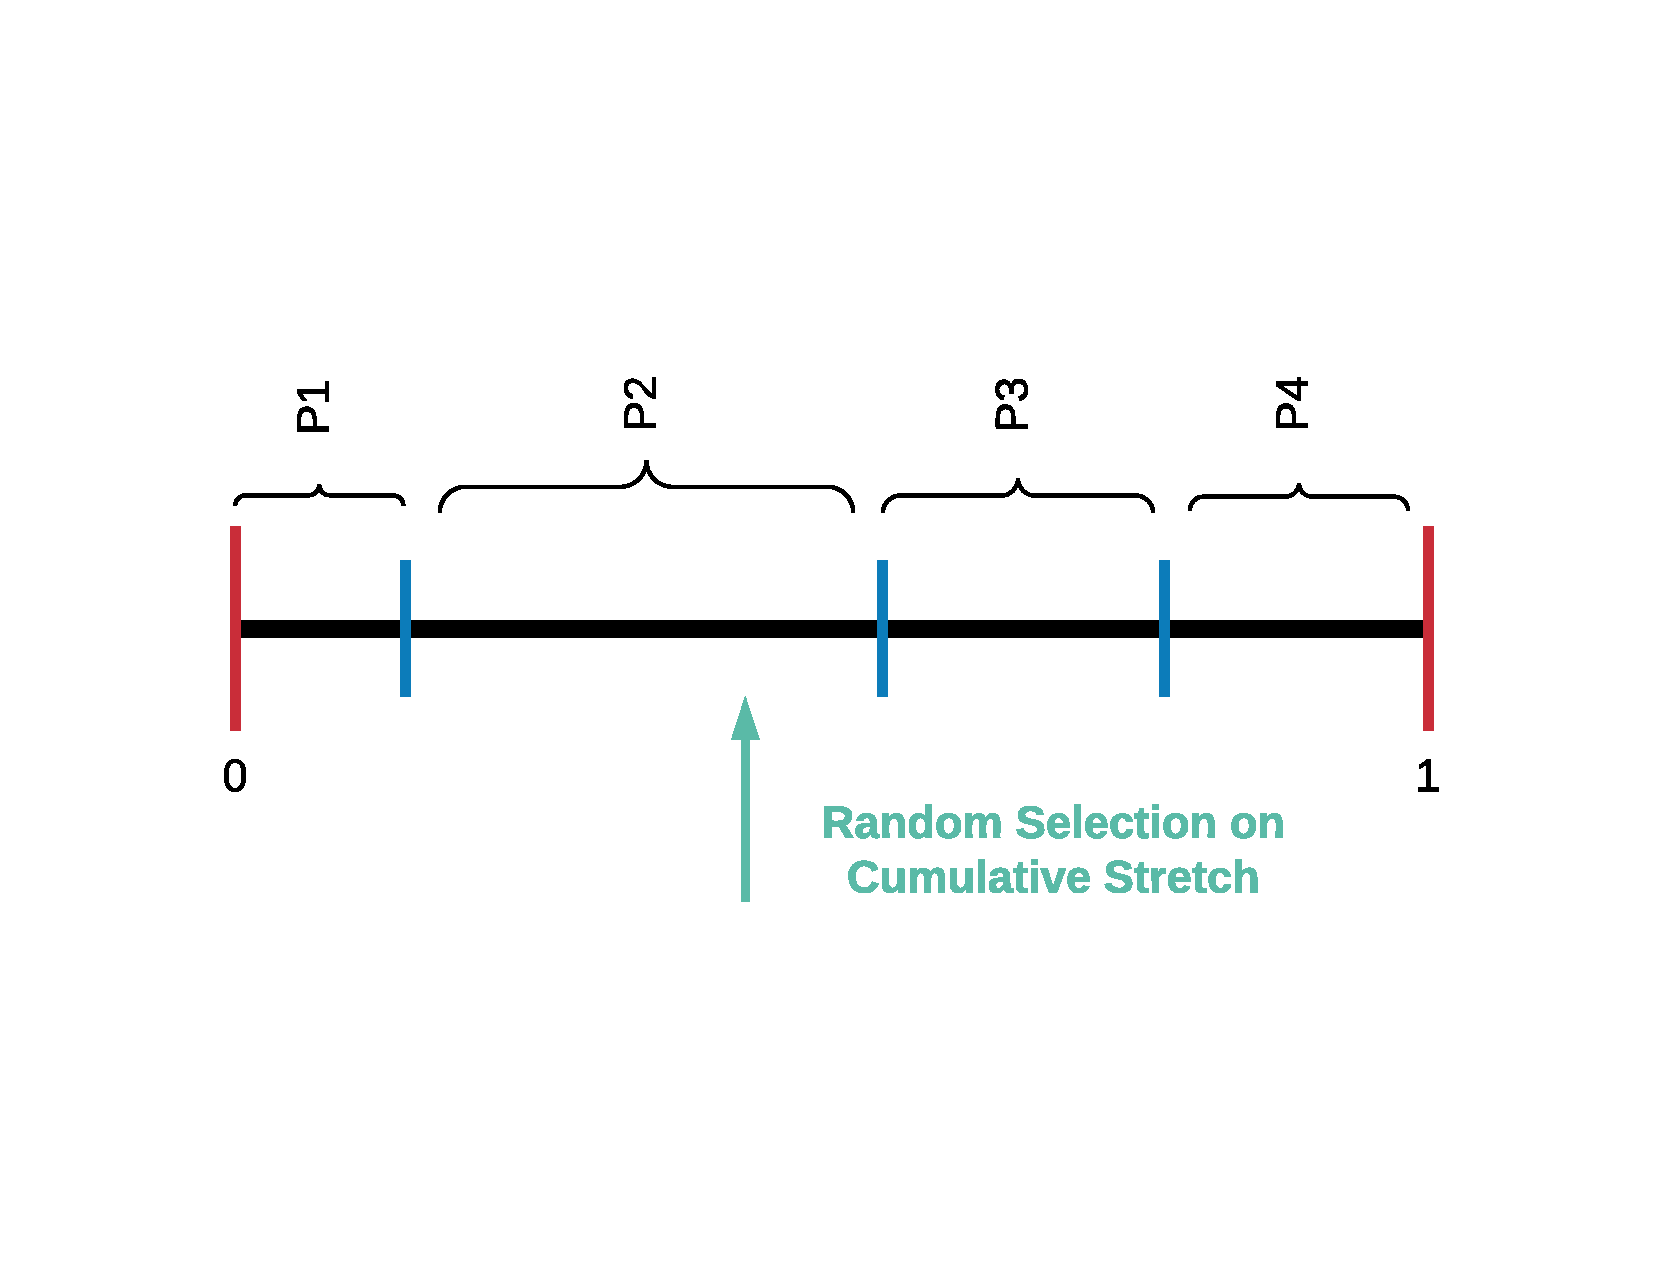
\includegraphics[width=0.7\linewidth]{graphics/Random_Gen}
	\caption{Random selection from a probability distribution}
	\label{fig:randomgen}
\end{figure}
Essentially, each probability in the distribution was put into bins corresponding to their size (as with P1, P2, P3 \& P4 in Figure \ref{fig:randomgen}).  With this setup in place, a random number was generated from the uniform continuous distribution, and the probability bin to which this number corresponded was selected as the next character in the sequence.  This system self-propagates itself; each new character produces a new bigram on which to base the next random generation.  The first bigram was set to always be a `\#' followed by a random character.\\
\hfill\break
Whenever a `\#' is generated, this signifies a line break (as explained in the answer to Question \ref{PreProc}).  Thus, the system was set to automatically add another `\#' when this occurs, signifying both the end of a line and the start of a new one.  The next output character in the sequence will then be based on a `\#\#' bigram.  This system works for both the Europarl and given model.  The extra `\#' is of course not included in the count of random characters.\\
\hfill\break
The random generation process has also been summarised in pseudocode, as shown in \\Algorithm \ref{RanGen}.


\begin{algorithm}[H]
	\caption{Random Generation}\label{RanGen}
	\begin{algorithmic}[1]
		\Procedure{generate\_from\_lm}{Num\_Chars, Model, Valid\_Char\_List}
		\State $sequence = []$
		\State $bigram\_in \gets  \text{`\#'} + random(Valid\_Char\_List)$
		\State $chars\_left \gets Num\_Chars -1$
		\BState \emph{loop}:
		\If {$chars\_left > 0$}
				\If {$bigram\_in[1] == \text{`\#'} \ and\  bigram\_in[0]\ !=  \text{`\#'} $}
				\State $sequence \gets sequence +  \text{`\#'} $
				\Else
				\If {$bigram\_in == \text{`\#\#'}  $}
						    \State $possible\_tris \gets [bigram\_in + Valid\_Char\_List[excluding\ \text{`\#'}]]$.
				\Else
						     \State $possible\_tris \gets [bigram\_in + Valid\_Char\_List]$.
				\EndIf
		     	\State $distribution \gets model[possible\_tris]$.
		     	\State $bins \gets cumulative\_sum(distribution)$
		     	\State $distribution\_pos \gets random\_bin\_select(bins)$
		     	\State $new\_sequence \gets pos\_tris[distribution\_pos]$
		     	\State $bigram\_in \gets new\_sequence[0:1]$
		     	\State $sequence \gets sequence + new\_sequence[2]$
		     	\State $chars\_left \gets chars\_left - 1$
		     	\EndIf
		     	\State \textbf{goto} \emph{loop}.
				
		\EndIf
		\State \textbf{return} $sequence$
		\EndProcedure
	\end{algorithmic}
\end{algorithm}


\subsection{Sample Outputs}
When generating 300 sample characters of output from both models, two sample outputs obtained are shown below (\textcolor{red}{NL} signifies a new line, all `\#'s have been removed):\\

Generated from the Add-One-Smoothing Model trained on `training.en':\\
\hfill\break
\textit{.wyouterentlsol popmple be opmum pareen willon wity.\textcolor{red}{NL}\\
	mfte stragnu\textcolor{red}{NL}\\
	th thesion an lk.ltqnqake shou hatin actiong the we mad onlaticlasted betterevicand theqqltese the tooving miss ted\textcolor{red}{NL}\\
	welv0comh.x.gfunalwcnme counat implound thinitate trat to shose und be cof wo st pe of goin inagend thas new orwgoodur\\}
\hfill\break
Generated from the given model, `model-br.en':\\
\hfill\break
\textit{me it you ch ons.\textcolor{red}{NL}\\
	the get doggir.\textcolor{red}{NL}\\
	mor hose.\textcolor{red}{NL}\\
	whaskis it.\textcolor{red}{NL}\\
	ok.\textcolor{red}{NL}\\
	theres so thes doings.\textcolor{red}{NL}\\
	okay.\textcolor{red}{NL}\\
	what thet doin.\textcolor{red}{NL}\\
	them sho some right.\textcolor{red}{NL}\\
	oks.\textcolor{red}{NL}\\
	he ill one.\textcolor{red}{NL}\\
	wast wally not put want there buchats.\textcolor{red}{NL}\\
	ye.\textcolor{red}{NL}\\
	righ thesnt.\textcolor{red}{NL}\\
	hos tope.\textcolor{red}{NL}\\
	his dog.\textcolor{red}{NL}\\
	im his truseen ther.\textcolor{red}{NL}\\
	low yout apeer a toor.\textcolor{red}{NL}\\
	yeah.\textcolor{red}{NL}\\
	spee to tin you dog this backlif}
\subsection{Comments}
\begin{itemize}
	\item  The given model has line breaks after nearly every full stop.  The Europarl model places line breaks after full stops much less.  This  is possibly caused by the small size of the test data used.  The Europarl model has not prioritized new lines after full stops enough, even though most line breaks come after full stops in the training data. 
	\item  The given model produces much more new lines than the trained model.  The Europarl model has been trained on a corpus containing many long sentences, which explains why its output contains many long sentences in turn.  For the given model, this could possibly signify the model was training on data from some poem or text containing many short sentences.
	\item The given model actually produces some coherent words, whilst the Europarl model produces many more jumbled up words.  Again, this could be a consequence of the small size of the data used.  Interestingly, the given model contains many words such as `toy', `dog', `pup', `boy' or `daddy'.  This again points to the training text for this model being based on some kid-friendly text, possibly with very few sentences to make reading easier.  Of course, this could also be some form of dialogue between a child and his parents.  The Europarl model occasionally produces words such as `important', which appear frequently within the text.
	\newpage
\end{itemize}
\section{Perplexity Computation - Question 5}
\label{S5}
Perplexity is a measure of how well a model can predict the characters within a text corpus.  Essentially, it shows how well a text file's contents are related to the probabilities stored within a model.  This section provides an analysis of the different languages model, and how it fares against familiar and unfamiliar types of inputs.
\subsection{Perplexity Computation}
The general equation for perplexity ($PP_{M}$) computation is shown in Equation \ref{PP}.
\begin{equation}\label{PP}
	PP_{M} = P_{M}\left( c_{1}.... c_{n}\right)^{-\frac{1}{n}}
\end{equation}
Where $P_{M}(...)$ is the product of the probability of each character($c_{i}$) in an input text, and $n$ is the total number of characters in the input.\\
\hfill\break
 Using direct probabilities, however, will result in numbers which are too small for proper representation on a computer.  Thus, a log system was used by converting the perplexity measure into a log perplexity measure as follows:
\[log\left(PP_{M}\right) = log\left(P_{M}\left( c_{1}.... c_{n}\right)^{-\frac{1}{n}}\right)\]

\[log\left(PP_{M}\right) = -\frac{1}{n}\times log\left(P_{M}\left( c_{1}.... c_{n}\right)\right)\]
\begin{equation}\label{logPP}
log\left(PP_{M}\right) = -\frac{1}{n} \sum_{i=1} ^{n}\left( log(P_{M}(c_{1})) + ... + log(P_{M}(c_{n})) \right)
\end{equation}
The result, Equation \ref{logPP}, can be easily converted back to the normal perplexity measure by taking the antilog of its value.  This system allows one to compute the perplexity without running into any numerical representation issues.  This system was implemented as a standalone function, along with a number of checks to deal with the double `\#' preprocessing and other inadmissible conditions.  
\subsection{Testing the Language Models}
The test document provided acts as being an `unseen' document, and should act as a good validation of the expected result for each language model, at least with an English text input.  Each language model with Add-One Smoothing was used to calculate the perplexity of the test document, with the results shown in Table \ref{TR} (the model file result has been added for comparison).
	\begin{table}[H]
	\centering
	\setlength\arrayrulewidth{1pt}
	\caption{\label{TR}Perplexity results on the English test file }
	\begin{tabular}{c  c }
		\hline
		\textbf{Language Model} & \textbf{Perplexity (4 decimal places)} \\
		\hline                     
	English& \textbf{8.8696}\\
	German & 22.9270 \\
	Spanish & 22.5249 \\
	Given & 22.0930\\
	\end{tabular}
\end{table}
Looking at these results, it is clear that from the three language models, the English model has found the test document to be the least perplex, and by a large margin ($\sim$13.5).  This should mean that, by analyzing a document with all three of the models, one should be able to easily infer the language of the test document by finding the outlier (and much lower) perplexity value.  Further perplexity tests were carried out on a Spanish \cite{FSpan} and German document \cite{GSpan}, the results of which are shown in Table \ref{SR}.

\begin{table}[H]
	\centering
	\setlength\arrayrulewidth{1pt}
	\caption{\label{SR}Perplexity results on Spanish and German test files }
	\begin{tabular}{c c c}
		\hline
		\textbf{Language Model} & \multicolumn{2}{c}{\textbf{Perplexity (4 decimal places)} }\\
		\hline
		  & \textbf{Spanish File} & \textbf{German File} \\
		\hline                     
		English& 22.6965 & 20.6750\\
		German & 29.3398 & \textbf{8.6951}\\
		Spanish & \textbf{11.3395} & 27.9311\\
		Given & 51.9747& 45.1458\\
	\end{tabular}
\end{table}

Again, the perplexity results show a clear indication towards the correct document language, with the margin of perplexity difference between the correct language and other languages being at least 11. 

\subsection{Document Language Determination}

Whilst using all three models in tandem results in a good language classifier, using just one model for classification does not, even just for detecting the model's trained language.  This is easy to confirm using just the two English models - the given model and the Europarl English model.\\
\hfill\break
Looking back at Tables \ref{TR} and \ref{SR}, the given and Europarl model perplexity results vary considerably.  In Table \ref{TR}, the Europarl model reports back a perplexity of $\sim$8 whilst the given model reports a perplexity of $\sim$22.  Taking the Europarl model by itself, one might think that it should be obvious that the test document is written in English.  However, had one used just the given model, one would think twice before deciding on the language!  It is entirely possible that the Europarl model could assign such a high perplexity to an English document too, if the document is written in a format very different (e.g. with very short sentences, with many slang words or with lots of extra punctuation marks) to the one it was trained on.\\
\hfill\break
It is clear that using just one model in isolation is not enough to determine the language of a document.  One would need models of all the other possible languages the document could be in, in order to correctly deduce the document language.  Furthermore, each language model should ideally be trained on the same style and format of corpus (or a translation of the same corpus) in order to make sure that the only difference between models is in the language, and not in formatting or context.  

\section{Extended Analysis - Question 6}
\label{S6}
\subsection{Exploring Other Smoothing Methods}
Throughout all previous section of this report, results have been quoted from an Add-One smoothed model trained on the given training files.  Whilst this has produced good results, generally the Add-One smoothing method is regarded as a pretty inaccurate method of smoothing trigram models.  Thus, we attempted to branch out and use other model estimation methods for building the language models, in an attempt to make the divide between model perplexities for a particular language even more clear.
\subsubsection{Add-Alpha Smoothing}
The natural step-up from Add-One smoothing is to attempt to use Add-Alpha smoothing.  In this change, the `1' is simply changed to $\alpha$, a variable parameter between 0 and 1 which allows one to vary the distribution of probability when smoothing.  Using Add-Alpha smoothing, the perplexity computation on the three test files (from Section \ref{S5}) was repeated for various values of $\alpha$.  The results are shown graphically in figures \ref{fig:alphachanges_english} - \ref{fig:alphachanges_spanish}.

\begin{figure}[H]
	\centering
	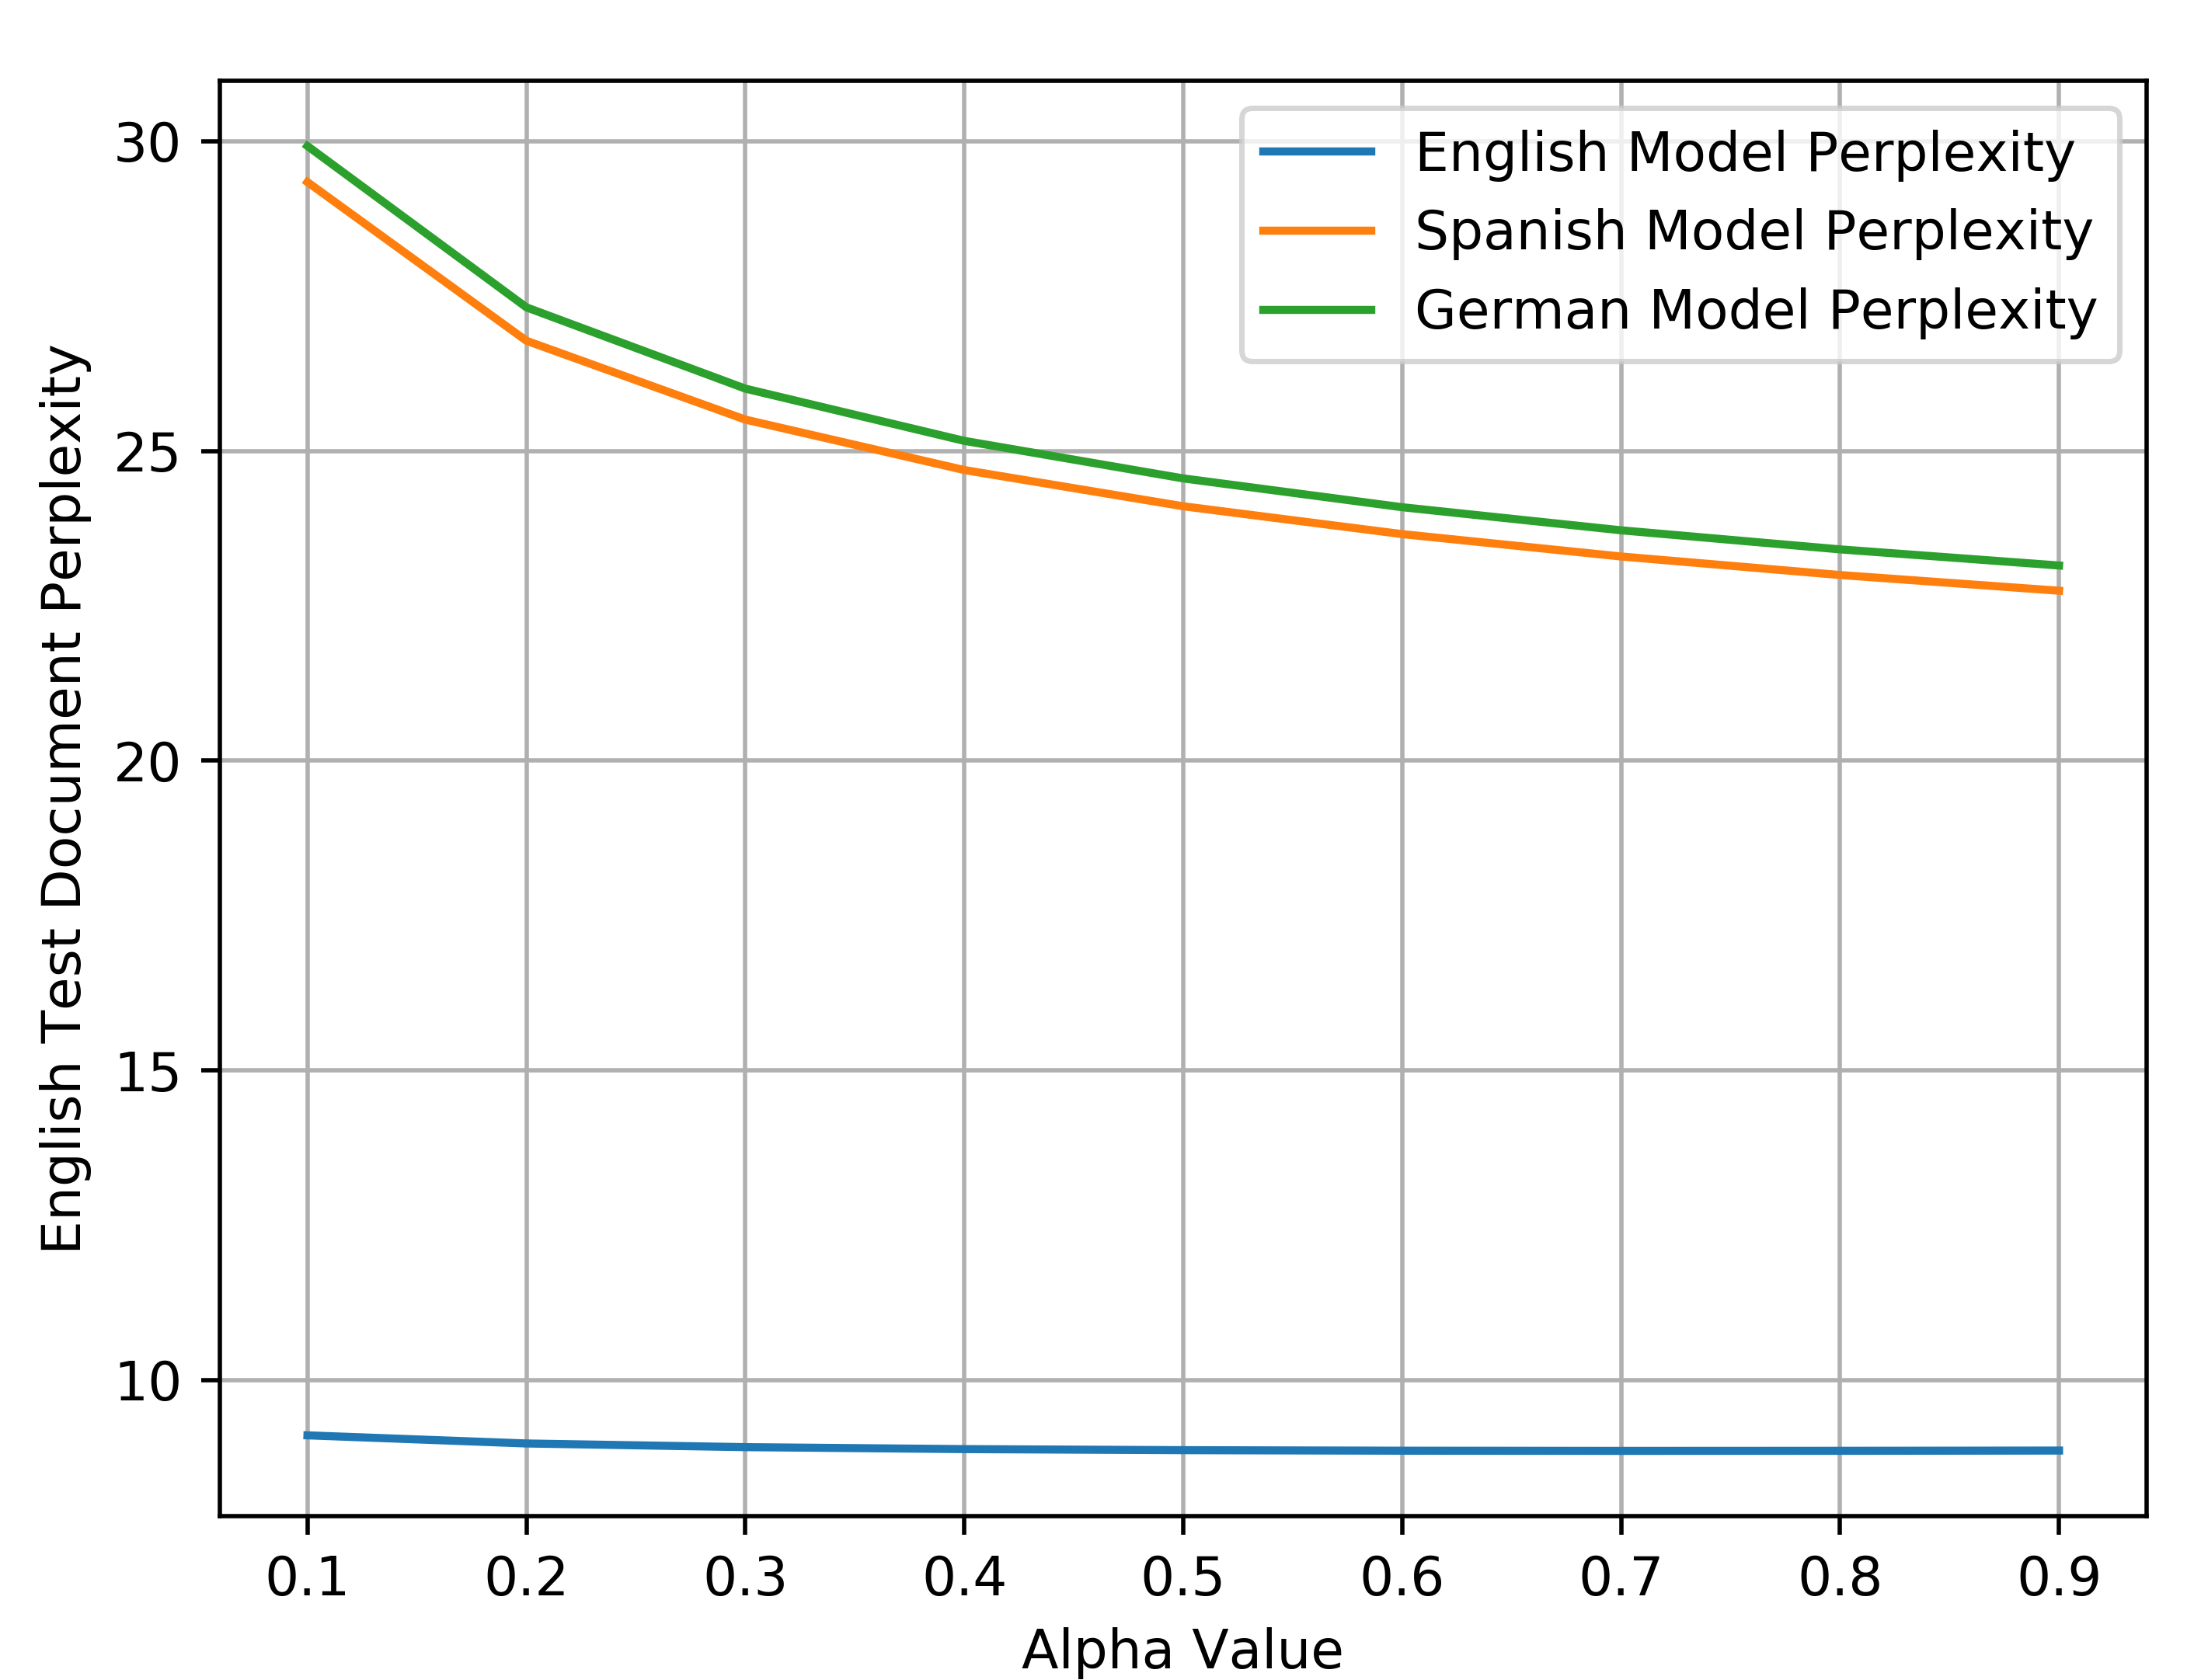
\includegraphics[width=0.7\linewidth]{graphics/alpha_changes_English}
	\caption{English test file perplexity results for different alpha values}
	\label{fig:alphachanges_english}
\end{figure}
\begin{figure}[H]
	\centering
	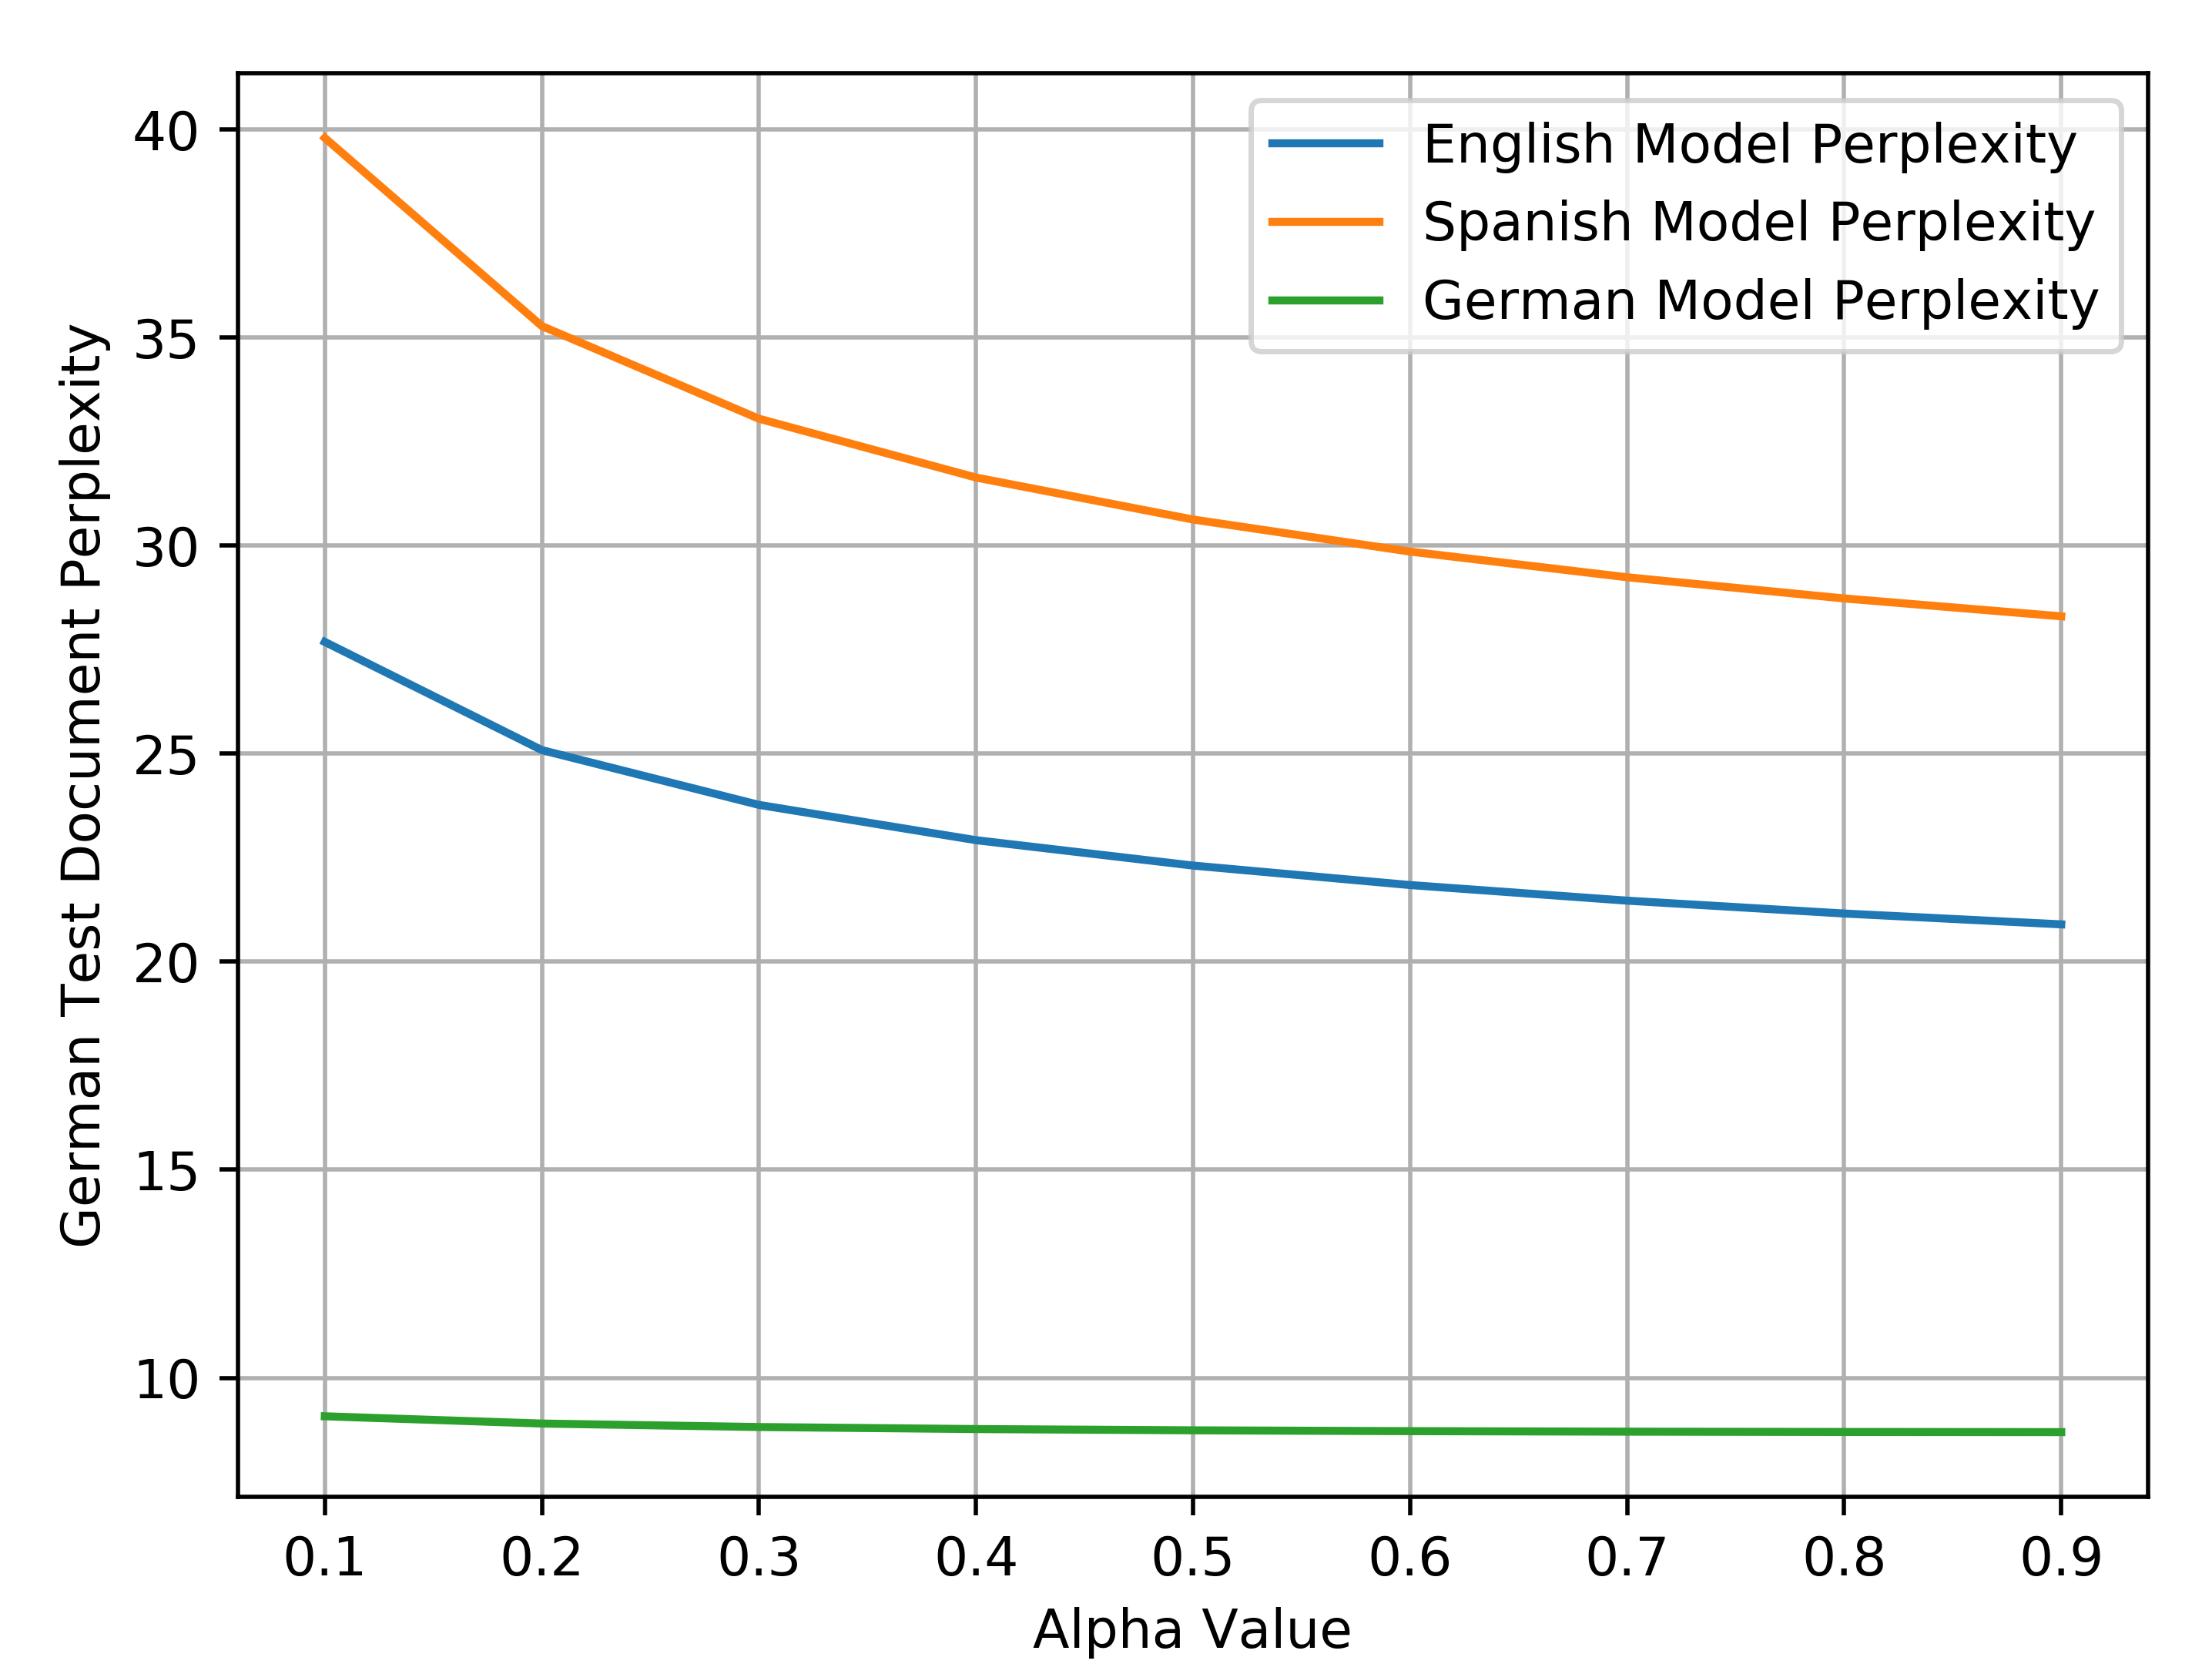
\includegraphics[width=0.7\linewidth]{graphics/alpha_changes_German}
	\caption{German test file perplexity results for different alpha values}
	\label{fig:alphachanges_german}
\end{figure}
\begin{figure}[H]
	\centering
	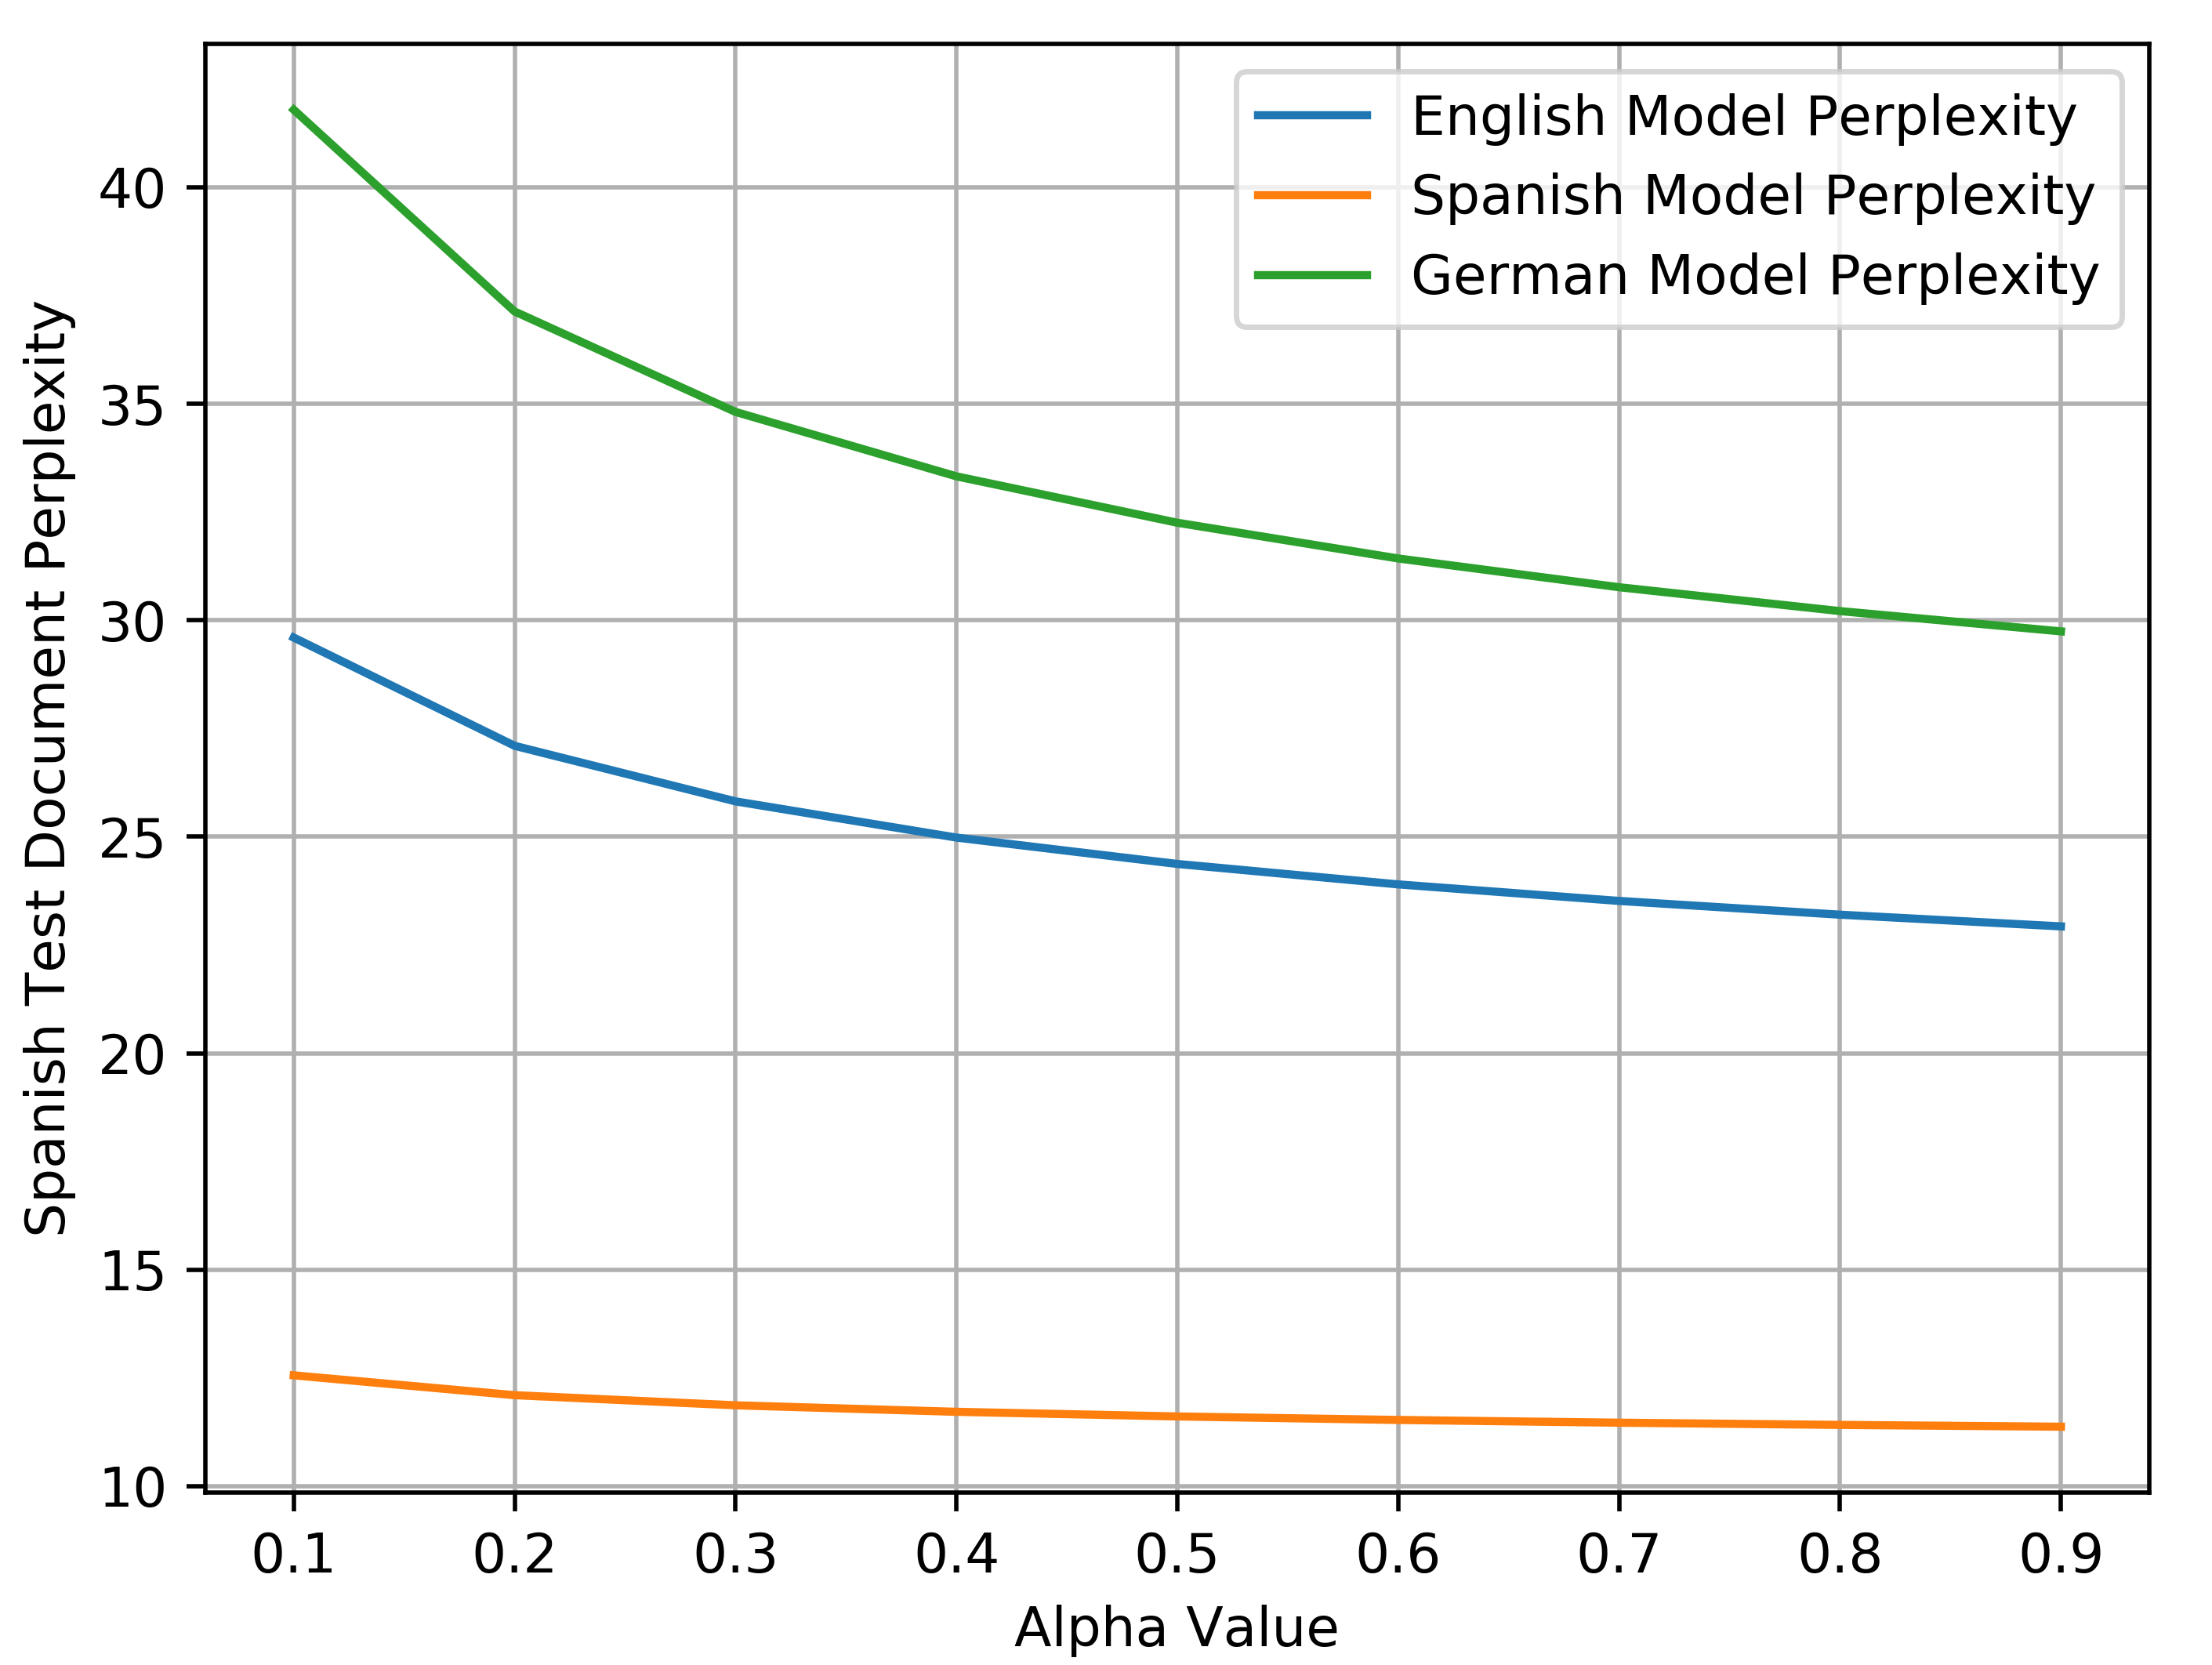
\includegraphics[width=0.7\linewidth]{graphics/alpha_changes_Span}
	\caption{Spanish test file perplexity results for different alpha values}
	\label{fig:alphachanges_spanish}
\end{figure}
From each graph, it is clear that the distance between the correct model's perplexity value and the rest of the models' perplexities increases as $\alpha$ decreases.  The changes are quite substantial, especially for the incorrect language models in each case.  However, the correct model's perplexity also increases slightly as $\alpha$ is decreased.  A possible explanation for this behaviour is that, with a lower $\alpha$, the models are being smoothed less drastically.  Thus, the models are slowly overfitting the training documents more and more as $\alpha$ is decreased.  The result of this is that the perplexity of unseen documents increases as the model is overfitting to the training data specifically, resulting in higher perplexities for documents which don't fit in exactly with the training files.\\
\hfill\break
 If choosing such a method of smoothing, one must ask whether it is preferred to have a larger gap for language classification, or have models cast a lower perplexity for documents of the same language.
\subsubsection{Interpolation}
Add-Alpha smoothing, whilst more customizable than Add-One smoothing, still assigns equal probability to unseen events.  An estimation method which avoids this is interpolation.  This method uses information from lower N-grams (bigrams and unigrams in this case) to attempt to assign more dynamic values to each unseen trigram probability.  The issue with the training data provided, however, is that many n-grams are never observed.  Thus, some form of uniform smoothing needs to be carried out on the data first before interpolation can be used (to ensure the distributions of each trigram is equal to 1).\\
\hfill\break
Thus, an interpolation scheme was built to use data from an Add-One smoothed trigram model, an Add-One smoothed bigram model and a Unigram model of the data.  Figure \ref{fig:interpchangesenglish} shows the perplexity results obtained from the three interpolated language models on the English test file.  The x-axis `iterations' refer to different combinations of the three underlying models (lambda values).
\begin{figure}[H]
	\centering
	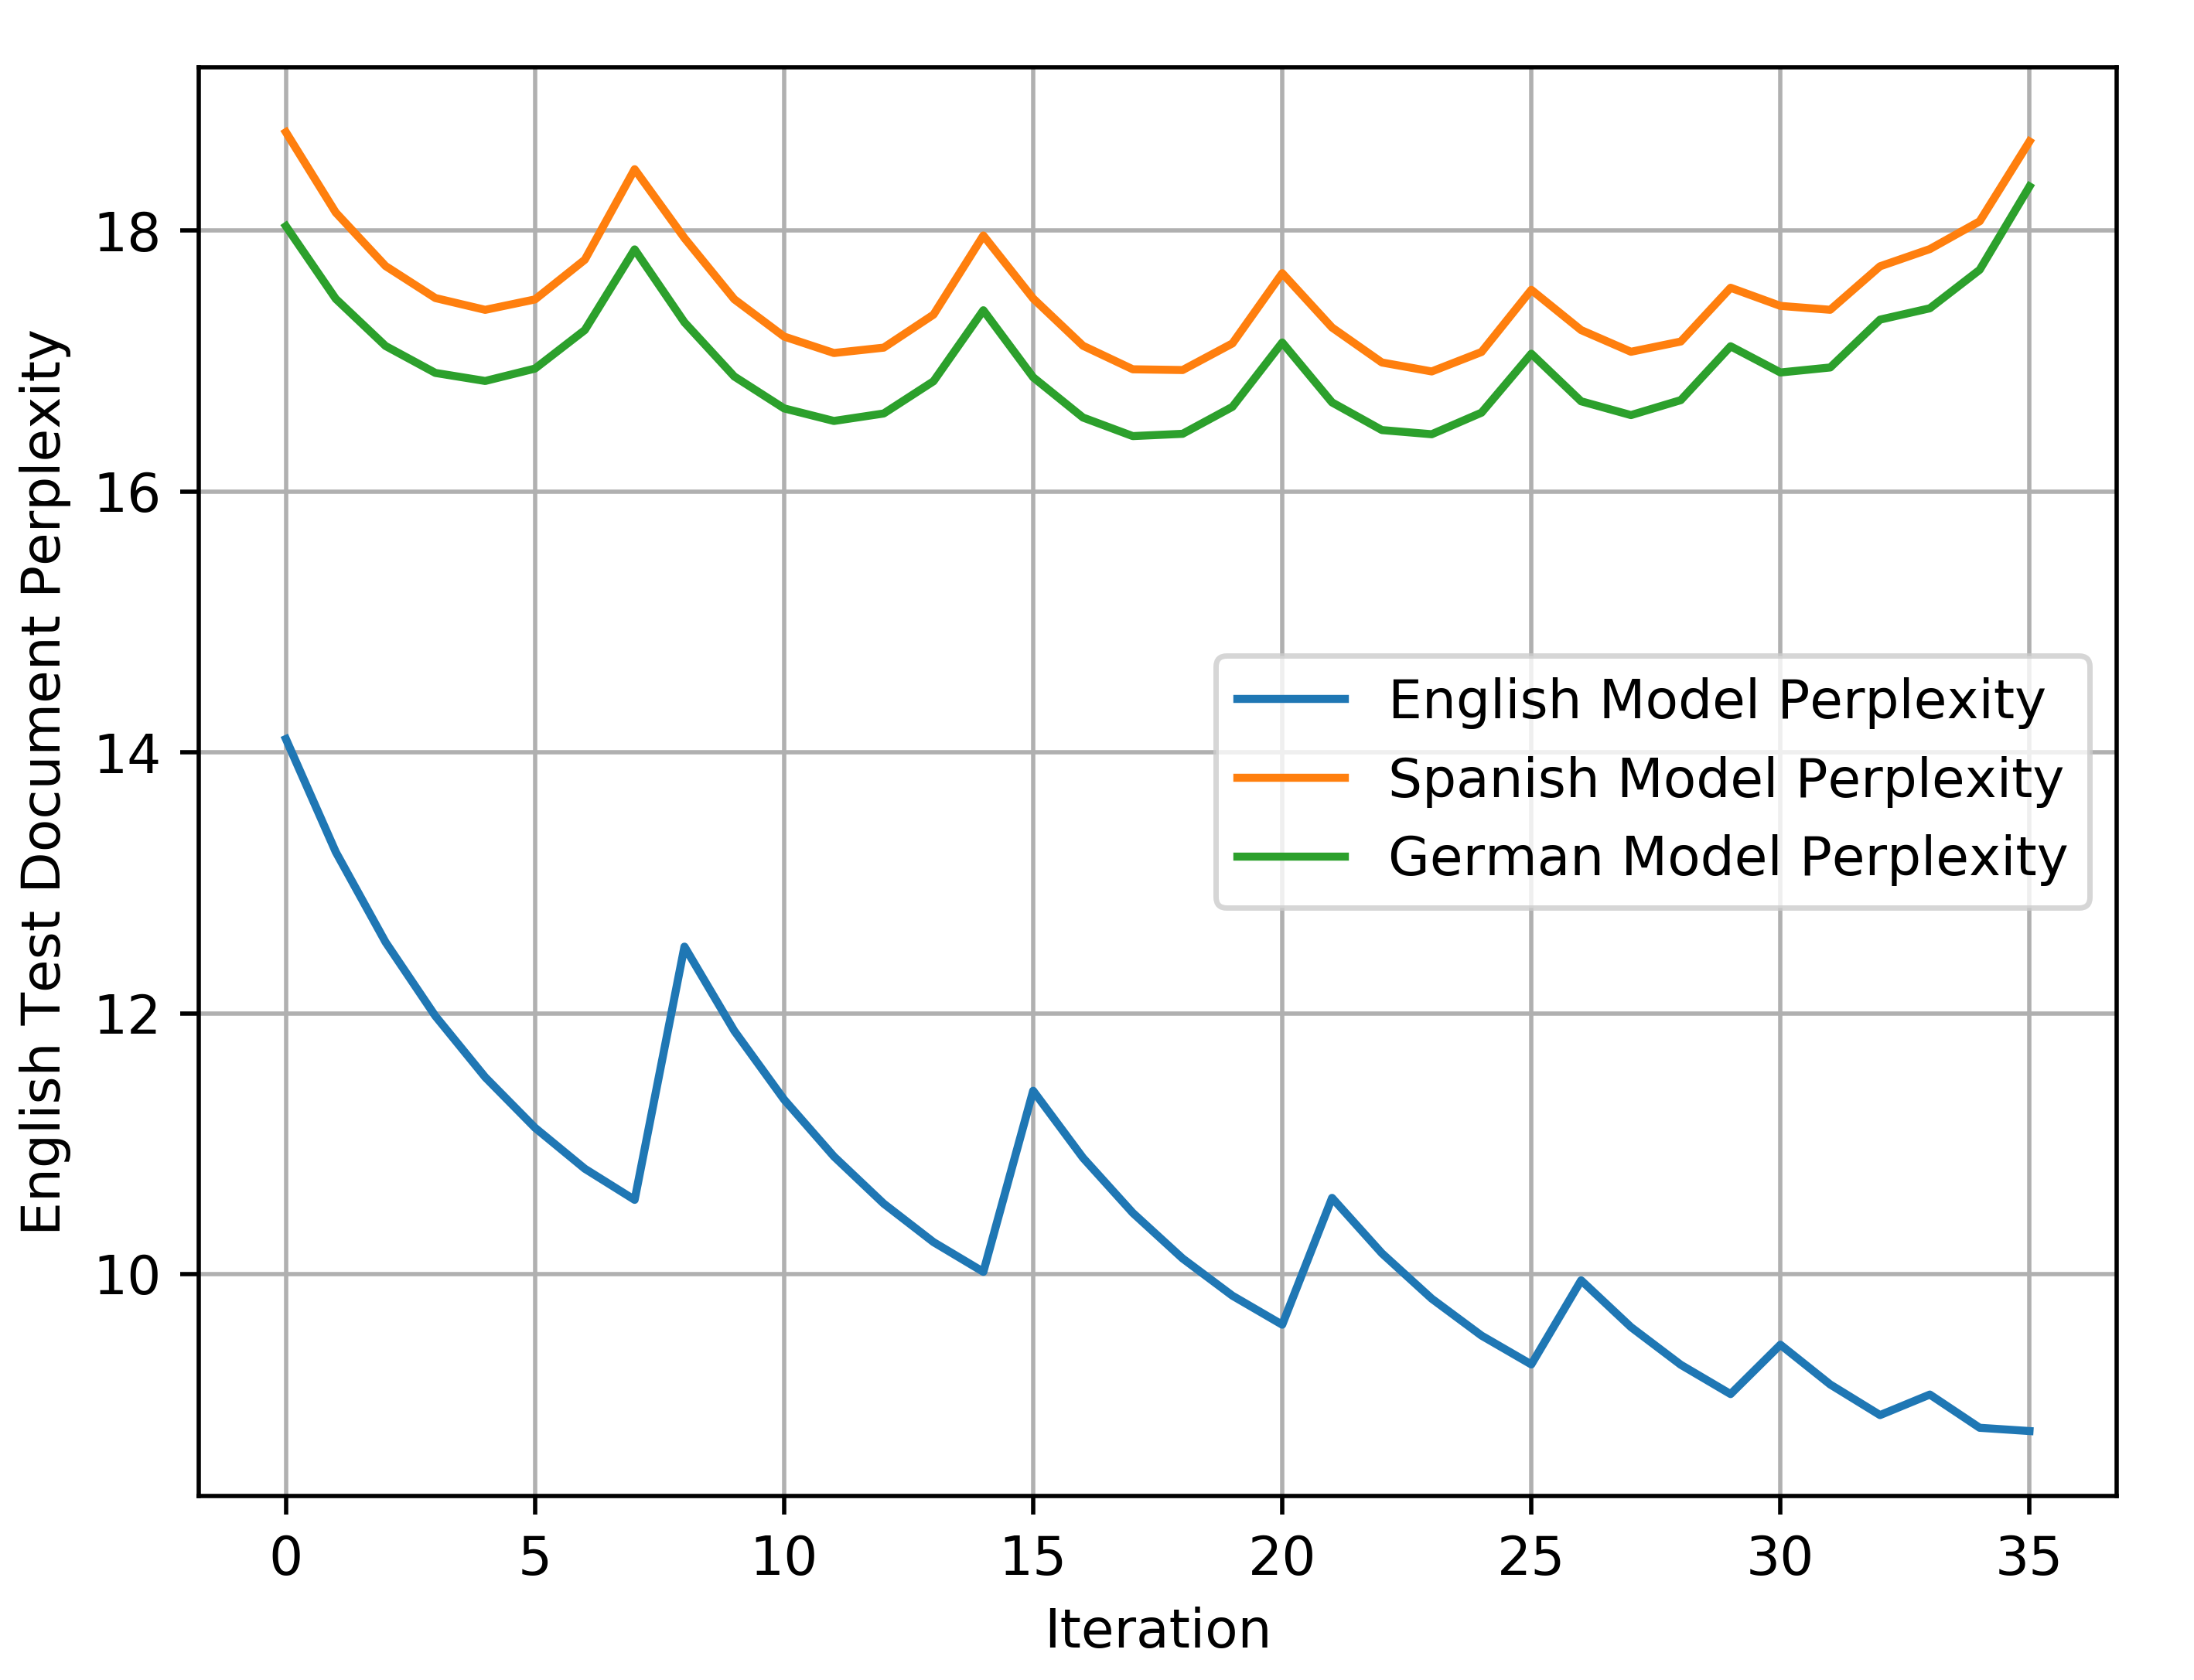
\includegraphics[width=0.7\linewidth]{graphics/interp_changes_English}
	\caption{Perplexity results for different interpolation parameters}
	\label{fig:interpchangesenglish}
\end{figure}
Unfortunately, as can be seen from the graph, the results of this method are worse for every combination of the three models (the same result has been obtained for the other test documents).  It seems that mixing-in information from lower models in this case results in perplexities which are less spaced out between the different language models.  It is clear that this method of estimation suffers when faced with a very sparse dataset.  Additionally, interpolation is probably not meant to be used with smoothed models.

\subsubsection{Other Estimation Methods}
Whilst other more complicated estimation methods exist such as Good-Turing or Kneser-Ney, it would seem unlikely that they would aid much in this situation.  Both would suffer from the fact that there are some uniformly-unseen trigrams (such as `zz\_') which offer no context for other estimation methods to attempt a more accurate estimation.

\subsection{Using N-grams as Document Classifiers}
\subsubsection{Problem}
A further question which we attempted to investigate was whether the N-gram character models trained could actually be used as a `document classifier'.  A document classifier is a model which is capable of assigning a document a particular class e.g. sports, legal, entertainment etc.  Such classes could vary according to the particular application.\\
\hfill\break
To investigate such a question, one would have to follow a procedure along the following lines:
\begin{itemize}
	\item  Obtain and label a dataset of documents with the different classes selected.
	\item Preprocess data to remove any metadata.
	\item  Split dataset into training/validation/testing sets.
	\item  Train N-gram character models on training set.  Use the resulting probabilities for each N-gram as a set of modeling features.
	\item  Feed in these data features to a logistic classifier.
	\item  Train classifier to identify different document types.
	\item  Model hyperparameters on validation set, and report final classification performance from test set. 
\end{itemize}
However, such a system would contain an enormous amount of features and parameters, requiring complex classifiers to attempt to fit the input data, as well as very large datasets.  Thus, instead, we attempted to discriminate between different classes through the use of the models trained in the previous sections of the assignment.  
\subsubsection{Classification Attempts}
The main measure we attempted to use to classify a document was it's perplexity under a particular trigram model.  To attempt such a test, a section of the Gutenberg \cite{Gutenberg} corpus was obtained, containing books labelled with their respective authors.  We first attempted to set out some method to classify a book according to its author, using different writing styles as a means of discriminating between different documents.\\
\hfill\break  
Before making an attempt at classification, the Europarl Add-One trigram model was used to compute the perplexity of every document (3036) downloaded from the dataset.  The average perplexity of these documents classified by author is shown in Figure \ref{fig:authorsper}.
\begin{figure}[H]
	\centering
	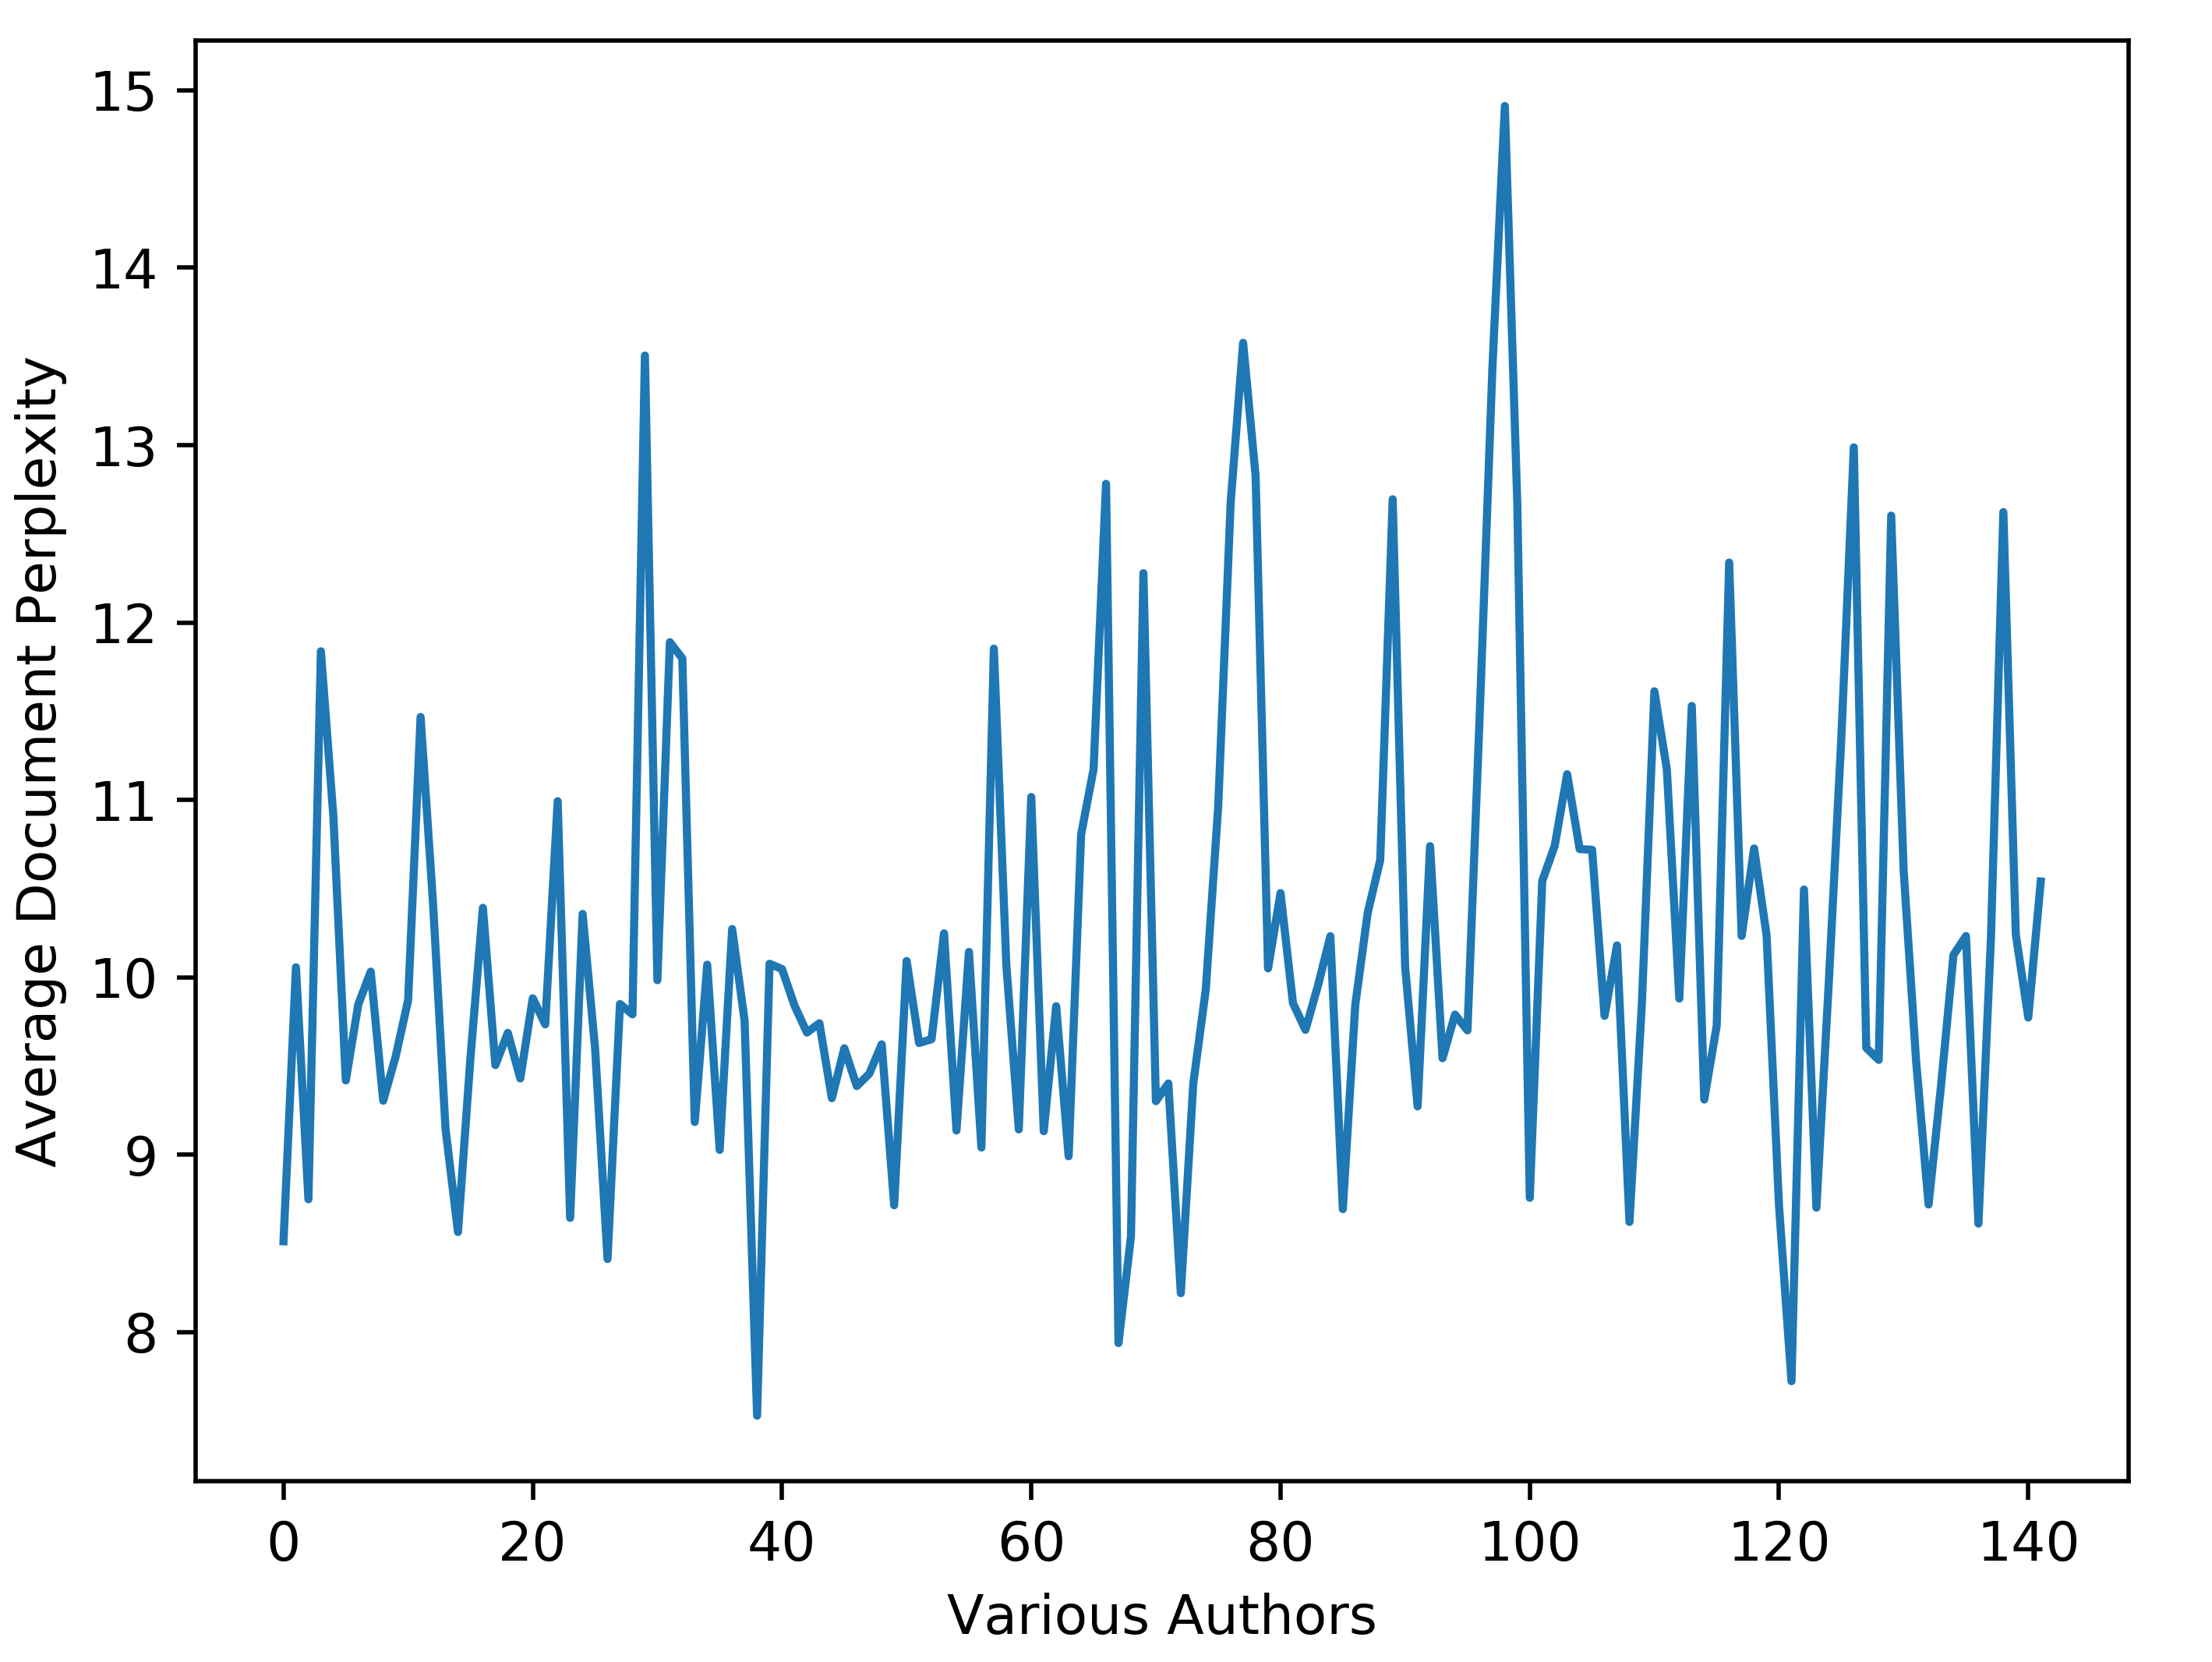
\includegraphics[width=0.8\linewidth]{graphics/authors_per}
	\caption{Perplexity results for a range of documents, with a total of 142 authors}
	\label{fig:authorsper}
\end{figure}
As can be seen from the graph, finding any trend relating document perplexity to the author will be very difficult!  There is nearly no chance that a classifier could be fitted on this data, with just the perplexities obtained from one trigram model.  A better bet at classifying this data would be through the use of a variety of trigram models, each computing their own perplexity values from the dataset.  Additionally, manual preprocessing of the data to remove headers, captions etc. would have been required to completely remove misleading data from the documents.\\
\hfill\break
As a final attempt at using the Europarl model as a document classifier, another dataset \cite{friends} containing the scripts for a popular drama series was downloaded.  This dataset contains English which is entirely different in style to that used in the Gutenberg corpus (most of the authors in the Gutenberg corpus lived in the 1800s).  The perplexities of the drama series episodes were also calculated using the Europarl model, and plotted on top of the Gutenberg perplexities, with the result being shown in Figure \ref{fig:authorsvsfriends}.

\begin{figure}[H]
	\centering
	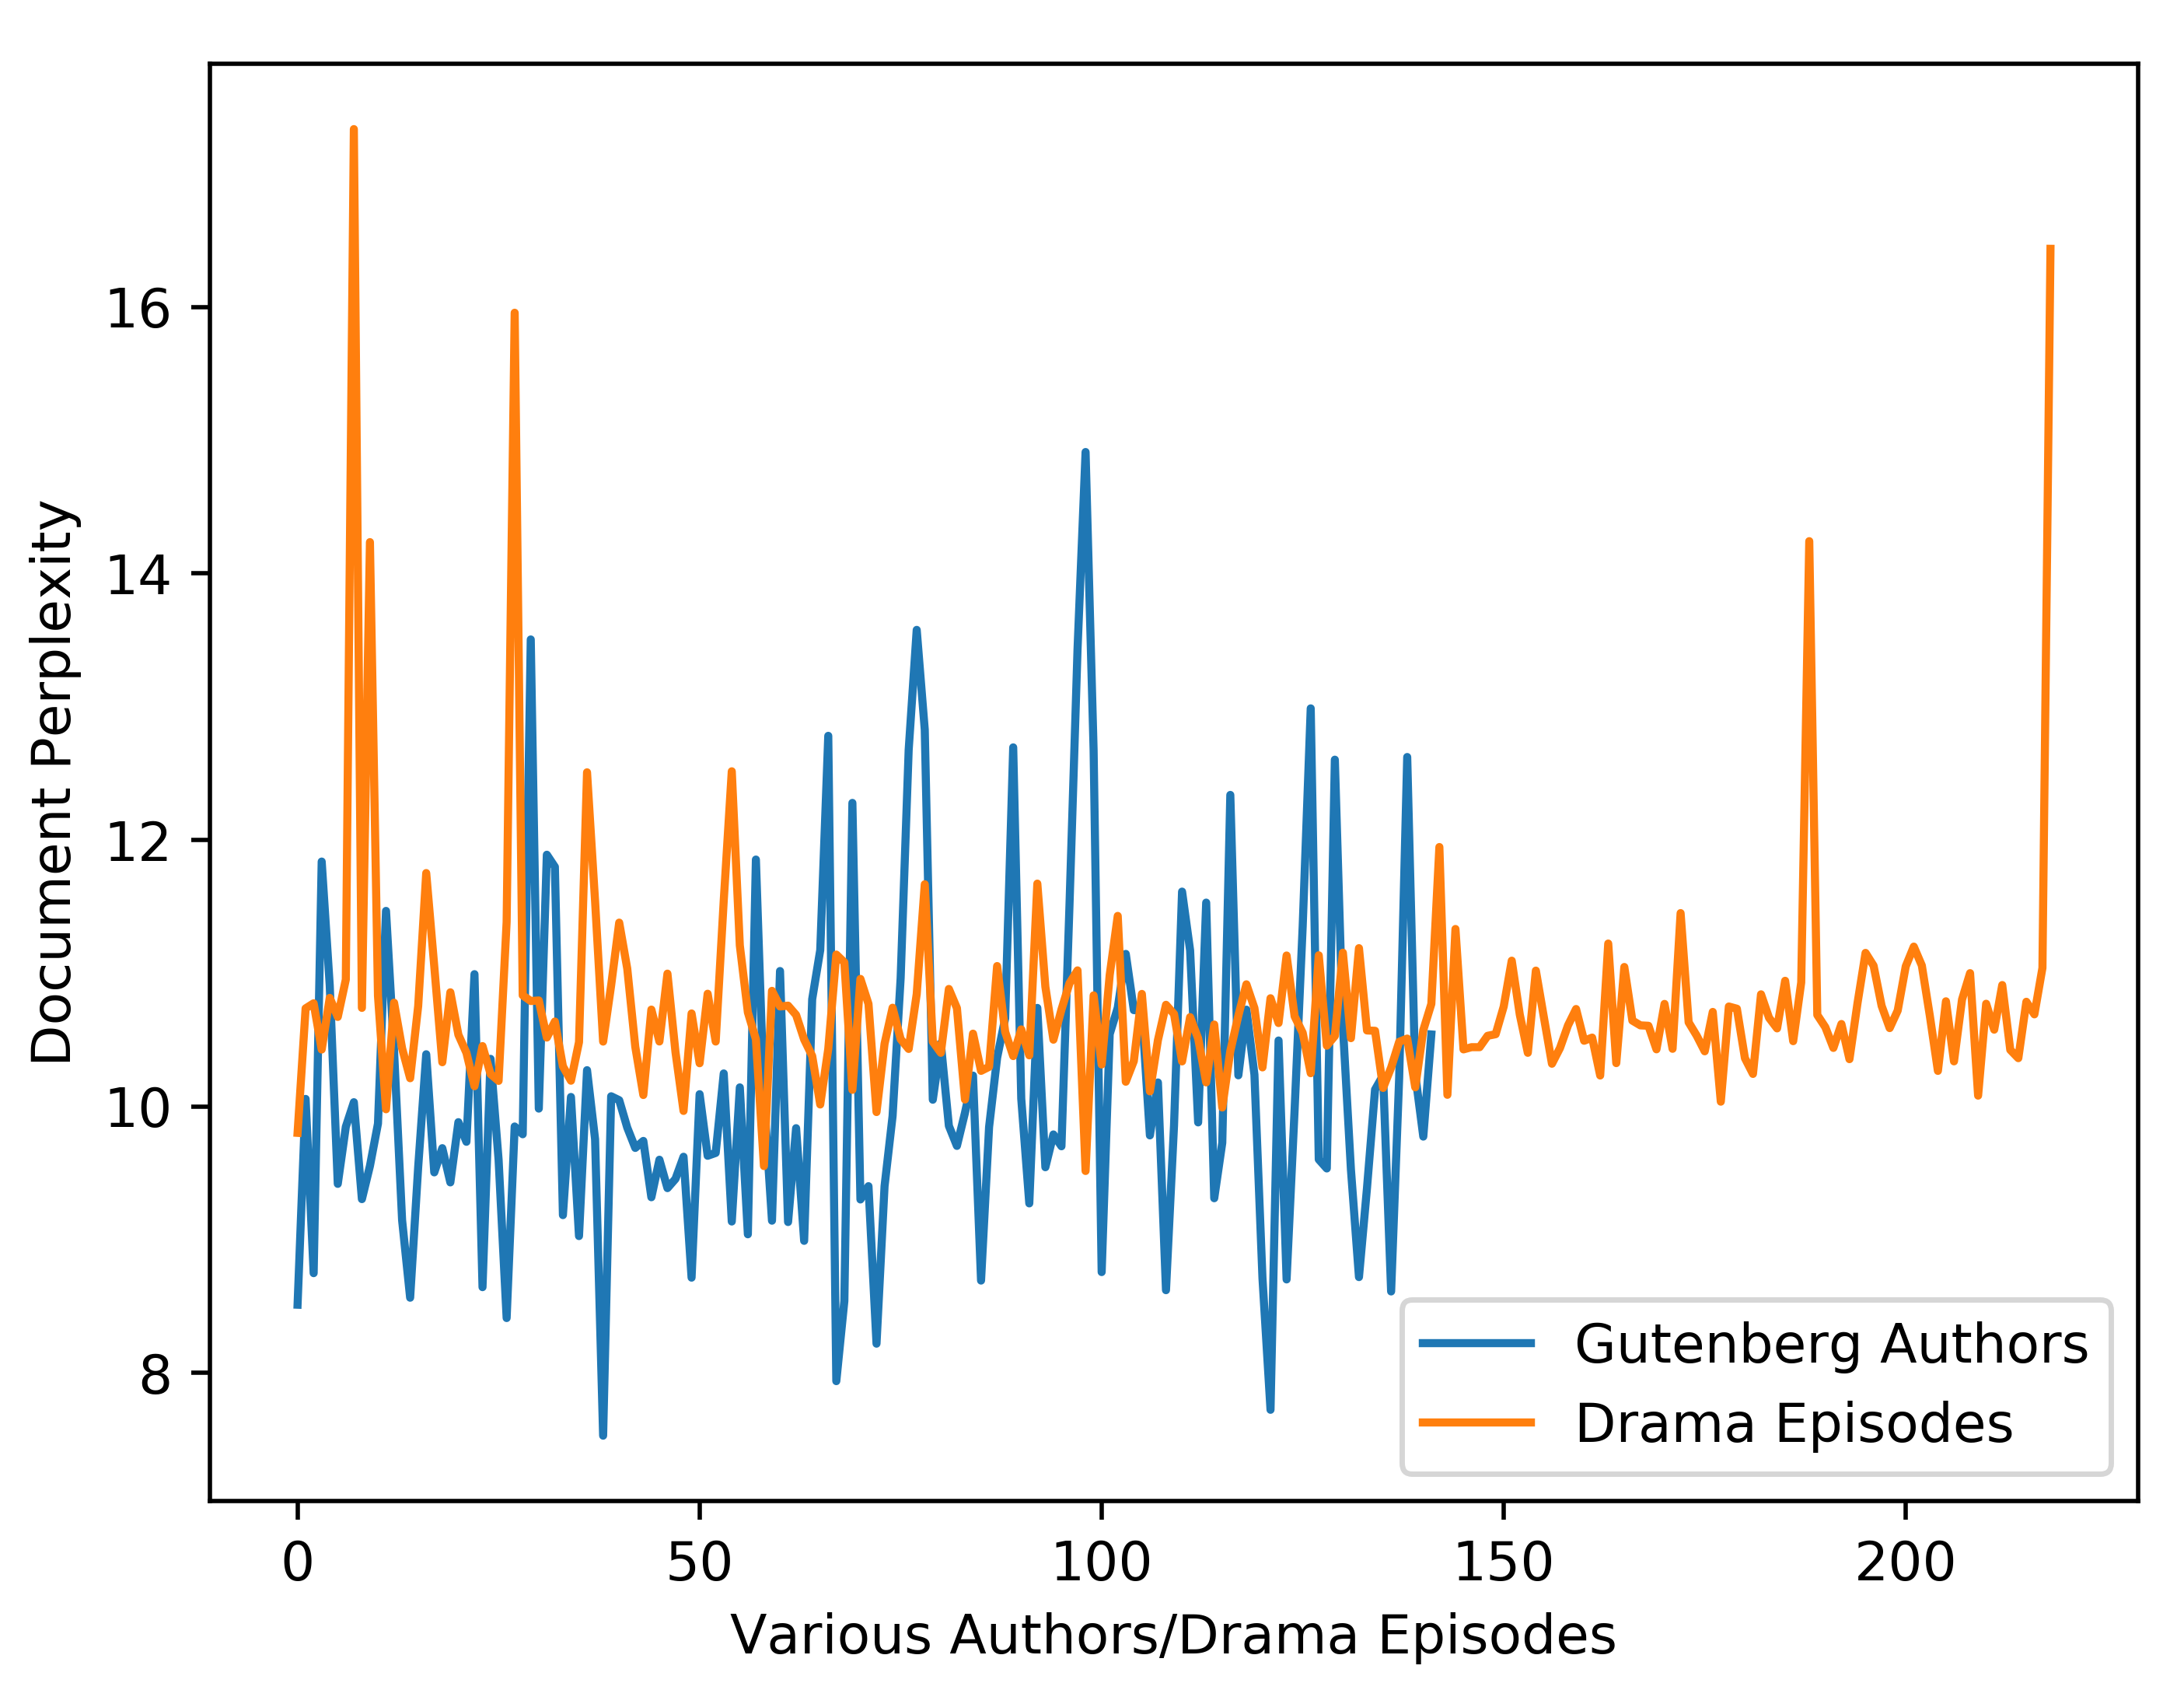
\includegraphics[width=0.8\linewidth]{graphics/authors_vs_friends}
	\caption{Perplexity results for two datasets}
	\label{fig:authorsvsfriends}
\end{figure}

Again, the perplexity results appear entirely random.  Little or no difference is present between the two datasets, other than the fact that the drama episodes' perplexities are more tightly packed at a central value than the other dataset.  As before, it would be very difficult to fit a classifier based on these perplexity values.\\
\hfill\break
This exercise has concluded that using a simple trigram model to classify documents is not in fact an easy task!  Language classification is much easier given the big differences between the character content in different languages.  A more complex model capable of capturing the style and form of a document's text would ideally be required for document classification.  However, it could also be possible that through the use of many N-gram models simultaneously, one could still be able to extract some useful information from the datasets (albeit requiring a more complex and computationally expensive system).

\section{Conclusions}
Throughout this assignment, various methods for generating character-level trigram models have been explored.  Whilst their limits and issues have been thoroughly explored, the built models have been used to successfully identify document languages by computing the document's perplexity.  An attempt has been made to extend the models to act as document classifiers, however poor results have been obtained.  Such an application would require further exploration and analysis for the trigram models to successfully act as document classifiers.

\begin{thebibliography}{4}
	\bibitem{FSpan}  Friends Script Spanish Translations: https://www.friendspeich.com/guiones01.php
\bibitem{GSpan}German Text Source: https://lingua.com/german/reading/
\bibitem{Gutenberg} Gutenberg Corpus used: http://web.eecs.umich.edu/$\sim$ lahiri/gutenberg\_dataset.html
\bibitem{friends} Drama Corpus: https://github.com/nlp-compromise/nlp-corpus
\end{thebibliography}

\end{document}
